
\documentclass[sigconf]{acmart}
%%
%% \BibTeX command to typeset BibTeX logo in the docs
\AtBeginDocument{%
  \providecommand\BibTeX{{%
    Bib\TeX}}}

\usepackage{tikz}
\usepackage{pgfplots}
\usepackage{verbatim}
\usepackage[utf8]{inputenc}
\usepackage{placeins}
\usepackage{enumitem}
\usepackage{titlesec}
\titlespacing*{\section}{0pt}{0.5em}{0.5em}

\usetikzlibrary{calc}
\settopmatter{printccs=false}
\settopmatter{printacmref=false}
\usepackage{pgfplots}
\pgfplotsset{compat=1.18}  % or latest installed version
\usepackage[font=small,skip=2pt]{caption}
\settopmatter{printacmref=false}   % no "ACM Reference Format" box under title
\setcopyright{none}                % hide the permissions/copyright footer
\acmDOI{}
\acmISBN{}
\acmYear{}
\copyrightyear{}
\acmConference{}{}{}               % (series, date/location all empty)

\pagestyle{plain}

% Belt-and-suspenders: in case a leftover footnote would appear
\makeatletter
\renewcommand\footnotetextcopyrightpermission[1]{}
\makeatother


\begin{document}

%%
%% The "title" command has an optional parameter,
%% allowing the author to define a "short title" to be used in page headers.
\title{Group 6: Final Report}

%%
%% The "author" command and its associated commands are used to define
%% the authors and their affiliations.
%% Of note is the shared affiliation of the first two authors, and the
%% "authornote" and "authornotemark" commands
%% used to denote shared contribution to the research.
\author{Jun Tang}
\affiliation{%
  \institution{Fairleigh Dickinson University}
  \city{Vancouver}
  \country{Canada}
}
\email{j.tang4@student.fdu.edu}

\author{Xiaoyi Han}
\affiliation{%
  \institution{Fairleigh Dickinson University}
  \city{Vancouver}
  \country{Canada}
}
\email{x.han1@student.fdu.edu}

\author{Kaiwen Wang}
\affiliation{%
  \institution{Fairleigh Dickinson University}
  \city{Vancouver}
  \country{Canada}
}
\email{k.wang4@student.fdu.edu}

\author{Ziyan Qiu}
\affiliation{%
  \institution{Fairleigh Dickinson University}
  \city{Vancouver}
  \country{Canada}
}
\email{z.qiu1@student.fdu.edu}

\author{Hongyi Niu}
\affiliation{%
  \institution{Fairleigh Dickinson University}
  \city{Vancouver}
  \country{Canada}
}
\email{h.niu@student.fdu.edu}


\renewcommand{\shortauthors}{}   % clear the short author string
\fancyhead{}                     % clear all header fields (acmart uses fancyhdr)

%%
%% The abstract is a short summary of the work to be presented in the
%% article.
\newif\ifprintabstract
\printabstractfalse   % set to \printabstracttrue if you want it

\ifprintabstract
\begin{abstract}
To be added later.
\end{abstract}


\begin{CCSXML}
<ccs2012>
 <concept>
  <concept_id>00000000.0000000.0000000</concept_id>
  <concept_desc>Do Not Use This Code, Generate the Correct Terms for Your Paper</concept_desc>
  <concept_significance>500</concept_significance>
 </concept>
 <concept>
  <concept_id>00000000.00000000.00000000</concept_id>
  <concept_desc>Do Not Use This Code, Generate the Correct Terms for Your Paper</concept_desc>
  <concept_significance>300</concept_significance>
 </concept>
 <concept>
  <concept_id>00000000.00000000.00000000</concept_id>
  <concept_desc>Do Not Use This Code, Generate the Correct Terms for Your Paper</concept_desc>
  <concept_significance>100</concept_significance>
 </concept>
 <concept>
  <concept_id>00000000.00000000.00000000</concept_id>
  <concept_desc>Do Not Use This Code, Generate the Correct Terms for Your Paper</concept_desc>
  <concept_significance>100</concept_significance>
 </concept>
</ccs2012>
\end{CCSXML}

\ccsdesc[500]{Do Not Use This Code~Generate the Correct Terms for Your Paper}
\ccsdesc[300]{Do Not Use This Code~Generate the Correct Terms for Your Paper}
\ccsdesc{Do Not Use This Code~Generate the Correct Terms for Your Paper}
\ccsdesc[100]{Do Not Use This Code~Generate the Correct Terms for Your Paper}

%%
%% Keywords. The author(s) should pick words that accurately describe
%% the work being presented. Separate the keywords with commas.
\keywords{Cache, Admission policy, Flash drive, Machine Learning}
%% A "teaser" image appears between the author and affiliation
%% information and the body of the document, and typically spans the
%% page.
\fi
\begin{abstract}
In modern era, data size for system in cloud increases so fast that the storage system has to handle exponentially increasing I/O access to backend storage system. Tradition hard disk drives (HDDs) is cost-effective but eventually can't fulfill the high volumn I/O demands and become the major bottleneck for the storage system. \textit{Baleen} (FAST~'24) utilized a machine learning–guided flash caching framework to improve the storage system and balance the cost of cache flash drives. Based on Baleen's work, our project reproduces and customize the eviction policy to evaluation and test the cache performance and the Peak Disk-head Time (Peak DT), median DT, hit rate, and flash write traffic. 

We implemented the DT-SLRU policy and Episode-Deadline Eviction (EDE) policy, and did a evaluation and ablation studies by controlling the parameters to analyze the impacts to the peak DT, median DT, hit rate parameters. Our test result reveals that changing the DT-SLRU promotion threshold ($\tau_{DT}$) and the EDE protected cap improve significantly the cache's performance with a threshold. Specifically, $\tau_{DT}\!\approx\!2$ and a protected cap near~0.5 have best perfromance where Peak~DT is reduced down to \textbf{45\%} relative to baseline. Our test demonstrates that tuning the eviction paramters will be very important for the cache system to deliver best performance.

\end{abstract}

%%
%% This command processes the author and affiliation and title
%% information and builds the first part of the formatted document.
\maketitle

%%\section{Introduction}
%%To be added soon
%%\clearpage

\section{Introduction}
Hard disk drives (HDDs) are still the main back bones of modern storage system as HDDs are affordable for storing huge amount of data \cite{akhtar2019avic}. But compared to the rocky-rising request on cloud application, HDDs storage system is too slow for servicing highly demanded system \cite{armenatzoglou2022redshift}. A single disk can sustain perhaps 100 requests per second \cite{beckmann2018lhd}. This will dramatically deter the system's performance in peak accessing time. Considering that not all data are equally needed by users, cache is a cheap way to resolve this challenge. Especially when the flash memory is available, add a flash drive cache before HDDs storage is a good strategy to improve the storage system's performance \cite{berger2017adaptsize}. By storing most commonly accessed data in cache, the system will be able response to data request far more faster and it prevents most of the load from happening in rush hours on our hard drives. While the existing flash memory has a fatal weakness that it can only be write for a fixed times. When it's been overwritten for a certain times, it has to be replaced for failure. As it’s expensive to replace flash, balancing between caching and saving cost is a key success aspect to pursure for engineering.

To achieve a good cache performance, typically, cache systems uses admission policies to load data into it \cite{chakraborttii2021flash}. The admission policies determine what data and when to put in the flash cache. CoinFlip\cite{belady1966replacement} and RejectX\cite{berger2018lightweight} are commonly used cache adminission policies. They are effective for good hit-rate, but they are not designed to minimize the writes to flash cache. Most of them attempt to achieve a higher hit rate or minimize the flash used. This means they are optimizing the cache cost for the system. These techniques do not address the worst-case delays from the disk drives and the cache cost balancing.

Many researches are attempting to use AI strategies to optimize the cahce system, balancing the hit-rate and the cache replacement cost. Baleen \cite{wong2024baleen} is one of the latest work to address this. Wong, et, al used machine learning in their cache strategy to determine what data is worth caching. They grouped the disk data requests into groups which they referred as episodes, and using baleen to train their model to predict which ones shave the most time. Then in their work, they used train models based on past data from these episodes, to implement admission policies and data prefetch policies. It then employs the models in simulation to lower peak load on hard drives. They quantified the system performance by Peak Disk-head Time (Peak DT). In their work\cite{wong2024baleen}, the authors minimize the peak DT, by prefetch policies to load data into flash cache. According to their test result, the cache system has better performance than other methods because it takes into account the data hit-rate and the falsh writting. 

Convential flysh cache additi plicnies Such as ondin Coinrip and RejectX relyonrandomization, or simple frsguMc yheuritirs io res- aboutthama writes on the Fash-storedsWrite by-pass synd ducts \cite{berger2014ttlnetworks}. For instance, RejectX defers blocks in such a way that the block is not admitted to program until being read several times; this helps avoid wasteful writes and extend flash storage life \cite{berger2018lightweight}. These strategies are simple and can be easily applied, but they depend on strict thresholds and coarse access patterns that are not able to cope with workload variety. Importantly, they do so primarily by optimizing flash wear or hit rates and ignore system-level performance characteristics, such as maximum backend load or disk head-time.

To overcome these shortcomings, ML has been investigated as a solution to enhance cache-related decisions by researchers. The Flashield system~\cite{eisenman2019flashield} proposed a DRAM-buffered flash cache with an ML classifier to predict reuse using only the DRAM access information. Likewise, CacheLib-ML \cite{berg2020cachelib} that runs in Meta used gradient-boosted decision trees with frequency and metadata features to filter flash cache admission. But both are designed for IO hit rate or bandwidth efficiency—not for disk-head time (DT), which is the bottleneck of high-throughput HDD- backed storage systems. They also did not include any long-term access correlation or lifetime costbenefit tradeoff.

The gap is covered by Baleen system \cite{wong2024baleen}, which presents a new cache residency model via episodes to better model access clusters across time. Baleen trains policy (supervised ML) to mimic an oracle admission pol-icy (OPT) which minimizes DT subject to flash write rate limits. In contrast with previous approaches, Baleen explicitly optimizes for Peak DT, which directly corresponds to the backend provisioning requirement. Furthermore, Baleen has been designed in modular form with decoupled admission, prefetching, and eviction modules making it feasible for a collective learning approach all the while maintaining explainability and system performance. In experimental testing on production traces, Baleen decreased peak backend load by 16\% and TCO for both immediately-served and backfilled requests by 17\% compared to the best baseline. 

Baleen already gives a strong base for cache research, but while working on it we still noticed some parts that feel not fully done yet. A lot of older works pay more attention to admission and prefetching, but not so much on eviction~\cite{wong2024baleen}. Things like parameter sensitivity or tuning were mentioned before, but not really tested deeply. Because of that, when workload changes or cache size becomes different, those systems sometimes behave weird or unstable. We think this kind of issue makes the system less flexible. So our main goal is to improve Baleen and try to make it perform more steady across different situations.

The idea is basically to let the system react faster when backend load changes. We mainly have two parts in our design: DT-SLRU (E1) and Episode-Deadline Eviction (E2). DT-SLRU changes its promotion threshold based on disk service time~\cite{beckmann2018lhd}, trying to find some balance between short-term reaction and long-term reuse. Episode-Deadline Eviction tries to guess how long each block might stay useful and gives it a soft “deadline” to remove it. It also keeps a small protected area for blocks with high DT-per-byte, since those are usually worth keeping longer. From what we’ve seen in early testing, the setup seems smoother and more consistent when workload becomes unstable.

Overall, our design shows that mixing ML-based guidance with temporal eviction can help the cache system stay stable and more adaptive to different workloads. It’s still not perfect, but already looks more reliable, especially when things get unpredictable or heavy.

Our contributions are summarized as follows:
\begin{itemize}[topsep=0pt, parsep=0pt, itemsep=0pt, leftmargin=*]
    \item We reproduce and extend the Baleen (FAST~'24) framework, focused on the underdeveloped eviction components in the ML-guided caching system.
    \item We implemented two adaptive eviction schemes --- DT-SLRU and Episode-Deadline Eviction (EDE).
    \item We performed ablation studies by adjusting the promotion threshold ($\tau_{DT}$) and protected-cap ratio, and examined how these parameters will affect Peak DT, median DT, hit rate, and flash write traffic.
    \item Our experiments shows that proper tuning of these parameters could lower Peak DT by around 45\% comparing to the baseline.
\end{itemize}


\section{Background}
\subsection{Flash Cache and Disk-head Time (DT)}

The speed of data growth is exponential \cite{turner2014digital}. Storage systems based on a hard disk drive (HDD) eventually fail to meet high-throughput requirements \cite{ren2019hybrid}.
According to \cite{luettgau2018survey}, on average, flash drives deliver 15--20 times the IOPS of hard disk drives and provide throughput 700--1000 times higher. Consequently, a modern storage stack is typically a layered system that serves client I/O requests through a hierarchy of devices. For cost considerations, it is still backed by HDD bulk storage, but to mitigate high I/O demand, a flash cache layer is placed in front to reduce peak backend load. The flash cache stages data in units of fixed-size segments, which allows it to spread out the cost of writing to flash while aligning with HDD read sizes for efficiency.  
The time for one HDD access consists of two parts: seek and move the head, and rotate the platter to read and transfer. The authors define Disk-head Time (DT) Eq.~\eqref{eq:dt-equation} where 
$t_{\text{seek}}$ is the average seek time and $t_{\text{read}}$ is the 
per-byte transfer time \cite{wong2024baleen}. 
\vspace{-0.5em} % adjust as needed
\begin{small}
\begin{equation}
DT_i = t_{\text{seek}} + n \cdot t_{\text{read}}
\label{eq:dt-equation}
\end{equation}
\end{small}

\begin{figure}[t]
    \vspace{-0.8em} % reduce space below
  \centering
  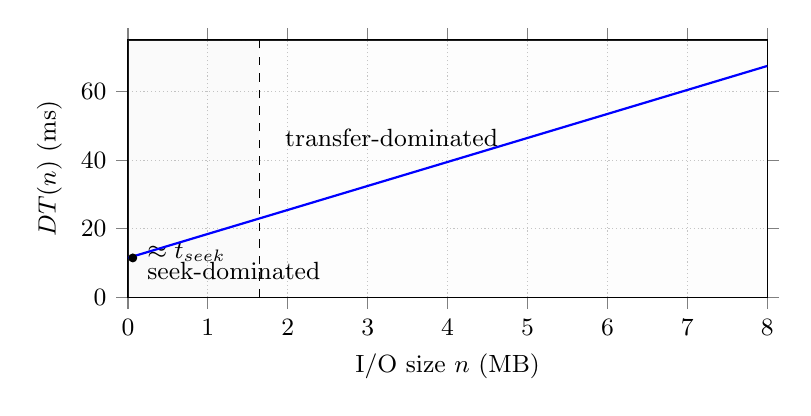
\begin{tikzpicture}
    \begin{axis}[
      width=0.8\columnwidth, height=0.4\columnwidth,
      xmin=0, xmax=8, ymin=0, ymax=75,
      xlabel={I/O size $n$ (MB)}, ylabel={$DT(n)$ (ms)},
      xmajorgrids, ymajorgrids, grid style={densely dotted},
      tick align=outside, tick style={thin},
      label style={font=\small}, tick label style={font=\small}
    ]

      % --- Paper constants (research testbed) ---
      \def\tseek{11.5}      % ms
      \def\bw{143.0}        % MB/s
      \pgfmathsetmacro\slope{1000/\bw}      % ms/MB  ≈ 6.99300699
      \pgfmathsetmacro\nstar{\tseek/\slope} % MB      ≈ 1.6445
      % --- Optional: light regime shading (draw FIRST) ---
      \addplot[draw=none, fill=gray!30, fill opacity=0.12]
        coordinates {(0,0) (\nstar,0) (\nstar,75) (0,75)} -- cycle;
      \addplot[draw=none, fill=gray!10, fill opacity=0.12]
        coordinates {(\nstar,0) (8,0) (8,75) (\nstar,75)} -- cycle;

      % --- Transition boundary ---
      \addplot[dashed] coordinates {(\nstar,0) (\nstar,75)};
      \node[anchor=south east, font=\small, align=right]
        at (axis cs:\nstar,72)
        {$n^\star \approx \pgfmathprintnumber[fixed,precision=2]{\nstar}\,$MB\\
         $t_{\text{seek}} = n^\star \cdot t_{\text{read}}$};
      % --- Labels + seek floor marker ---
      \node[anchor=north west, font=\small] at (axis cs:0.12,13) {seek-dominated};
      \node[anchor=north west, font=\small] at (axis cs:\nstar+0.2,52) {transfer-dominated};
      \addplot[only marks, mark=*, mark size=1.4pt] coordinates {(0.06,\tseek)};
      \node[anchor=west, font=\small] at (axis cs:0.12,\tseek+1.5) {$\approx t_{\text{seek}}$};

      % --- DT line (draw LAST so it’s on top) ---
      \addplot+[no marks, thick, samples=200, domain=0:8] {\tseek + \slope*x};
    \end{axis}
  \end{tikzpicture}
    \caption{DT vs.\ I/O size ($t_{\text{seek}}{=}11.5$\,ms, BW$=143$\,MB/s). 
    The line shows seek- and transfer-dominated regimes; 
    $crossover$ at $n^\star{\approx}1.64$\,MB. 
    Peak DT drives provisioning, which flash caching helps reduce.}
    \vspace{-1em} % reduce space below
  \label{fig:dt-one-line}
\end{figure}

This means HDDs have two constraints upon their throughput: IOPS (input/output operations per second) and sequential transfer bandwidth. Small I/Os are limited by IOPS, and large I/Os will hit the bottleneck of disk bandwidth. 

The authors emphasize DT ``balances IOPS and bandwidth'' and ``generalizes across variable-size I/Os'' \cite{wong2024baleen}. Regardless of request size, using DT as the unified optimization objective allows cache admission and prefetching policies to effectively reduce peak backend load on HDDs. ({Word count:} 252)

\subsection{Episode Model and OPT (Oracle)}
The episodes model groups related cache accesses together instead of tracking every single one individually, which makes flash caching analysis way more manageable. An episode is basically a bunch of accesses to the same data block that would all be hits if we decide to cache that block initially. The first access is always going to be a miss since the data isn't there yet, but everything else would be hits that can be efficiently served from the cache without additional disk activity.

They figure out episode boundaries using LRU eviction age. If two accesses happen within that time window, they are considered part of the same episode. If the gap is longer than eviction age, that’s where one episode ends and maybe a new one starts. This approach has nice advantages. Each episode can be analyzed independently, which makes the math way simpler. It also captures the main trade-off: you pay write cost upfront when caching data, then get benefits from hits during that episode, essentially trading flash endurance for reduced disk load.

The OPT policy uses this to approximate optimal decisions. It generates episodes using assumed eviction age, scores each episode by Disk-head Time saved per storage cost, then picks highest-scoring ones until the write budget runs out. Scoring formula:
\begin{equation}
\small
\label{eq:episode-score}
Score(\text{Episode}) = \frac{DT_{\text{Saved}}(\text{Episode})}{Size(\text{Episode})}
\end{equation}

What’s interesting is how it changes ML training. Instead of learning from individual accesses with complicated dependencies, models focus on episode-level decisions which is much simpler. The episode boundaries represent key decision points where you choose whether to admit something or not, and this abstraction makes model design far more tractable in practice. ({Word count:} 250)

\subsection{ML-Guided Admission (OPT Imitation for Peak DT)}
Machine learning--guided admission in flash caches refers to the use of a predictive model to decide whether a missed block should be inserted into cache under a constrained flash write budget. The approach is based on imitating an offline reference policy, OPT, which provides a near-optimal bound for maximizing disk-head time (DT) savings.

The training of this policy relies on the episode model, which groups all accesses to a block that would be hits if the block were admitted at the first access. Each episode is assigned a cost (number of flash segments written) and a benefit (total DT saved). Episodes are scored by their benefit-to-cost ratio as in Eq.~\eqref{eq:episode-score}.

Episodes are ranked by this score, and the highest scores are selected until the flash write budget is met. These selected episodes provide the labels used to train the admission model. The model is implemented as a binary classifier, typically using gradient boosting machines (GBMs). Input features include metadata describing the request context (namespace, user, block type) and dynamic features capturing recent access frequency. Samples from the first few accesses of each episode are included to capture early decision signals. The classifier outputs an admission probability, and a threshold is calibrated in simulation to achieve the desired flash write rate. The optimization target is Peak Disk-head Time, which reflects the highest backend load over a given interval. By focusing on DT rather than cache hit rate, the admission policy ensures that cache decisions reduce seek and transfer time, aligning with the objective of minimizing backend resource utilization.({Word count:}258)
\begin{figure}[h]
    \centering
    \includegraphics[width=0.85\linewidth]{episode-timeline.pdf} 
    \Description{Timeline of the episode model for a single block: showing cache-resident intervals (green), non-resident intervals, admissions (green arrows), evictions (red arrows), eviction age, and hits (black squares) annotated.}
    \caption{\textbf{Episode Model Timeline.} Two episodes of the same block are illustrated. Each episode begins with an \textbf{Admission} (green arrow), during which the block is \textbf{Cache-Resident} (green interval) and subsequent accesses are hits. If no access occurs for longer than the \textbf{Eviction Age}, the block is \textbf{Evicted} (red arrow), starting a \textbf{Non-Resident Interval}.}
    \label{fig:episode-timeline}
    \end{figure}

\subsection{ML-Guided Prefetching (Coordinated with Admission)}
ML-When is a classifier which aims to decide whether prefetching is worth executing for a given episode to achieve net reductions in DT \cite{wong2024baleen}. 
Based on the admission result made by Baleen's admission model, a binary classifier trained on episodes to imitate OPT \cite{wong2024baleen}---ML-Range proposes a contiguous segment range. ML-When then judges this proposal by estimating the marginal DT benefit of prefetching. If the predicted benefit is greater than a threshold (\(\varepsilon \approx 5 \,\text{ms}\), about half a disk seek), the prefetch is carried out; otherwise, it is skipped. By doing this, Baleen proactively caches the high-value segments of the data that are most likely to reduce the peaks in DT.
\begin{figure}[h]
    \vspace{-0.8em} % reduce space above
    \centering
    
\includegraphics[width=0.4\linewidth]{prefetch.drawio.pdf}
    \Description{Runtime workflow of Baleen system showing ML-Range and ML-When interaction for prefetching.}
    \caption{Runtime workflow of Baleen}
    \vspace{-0.6em} % reduce space below
    \label{fig:baleen-workflow}
\end{figure}
According to the paper, Baleen takes blocks (8 MB) as the data boundary. Within each block, the unit of data is a segment (128 KB). When an episode is admitted, ML-When evaluates ML-Range’s predicted segment range. If ML-When affirms the decision, those segments are prefetched and written into flash cache.
\begin{figure}[t]
    \vspace{-0.8em} % reduce space below
    \centering
    
\includegraphics[width=0.45\linewidth]{training-loop.drawio.pdf}
    \Description{Training loop for Baleen’s admission and prefetching models. 
    Runtime traces are labeled by OPT, then ML-Range and ML-When are trained to 
    approximate these labels for deployment.}
    \caption{Training loop for Baleen. Runtime traces are labeled with OPT; 
    ML-Range and ML-When are trained and deployed, producing new traces 
    to continue the cycle.}
    \vspace{-0.8em} % reduce space below
    \label{fig:training-loop}
\end{figure}

ML-When evaluates ML-Range’s proposals using the benefit formulas
(Eq. 3a–3e in \cite{wong2024baleen}), which quantify the DT saved by prefetching
versus not prefetching. If the predicted benefit exceeds a small threshold
($\varepsilon \approx 5$ ms, about half a disk seek), ML-When approves the
prefetch; otherwise, it is skipped. In this way, only high-value prefetches
are admitted, avoiding unnecessary flash writes.
({Word count:} 253)

\subsection{Baleen-TCO (Cost-Aware Flash Write-Rate Control)}

Total cost of ownership in Baleen was introduced as a consideration in cost controller mainly focused on balancing HDD cost and SSD endurance – more data request and transactions will occur on HDD directly if too little is written in SSD, raising cost due to affected performance costed by high peak DT and the demands for more HDD to maintain performance. Meanwhile, too much data written in the flash cache will accelerate abrasion on the SSD, which also increases cost.
\begin{figure}[H]
    \vspace{-0.8em} % reduce space above
    \centering
    
\includegraphics[width=0.7\columnwidth]{diagram.drawio.pdf} 
    \caption{Control Diagram}
    \Description{A control diagram with labeled inputs (TCO components, DT metrics) and outputs (target write rate).}
    \vspace{-1em} % reduce space below
    \label{fig:diagram}
\end{figure}
In this article, to address this issue, Baleen continuously monitors DT metrics (such as average DT and peak DT) as well as flash memory health metrics (such as remaining write cycles). Flash write rate was calculated dynamically to optimize the cache effect without overuse consumption of flash memory. Baleen achieved a trade-off that minimizing the TCO by protecting flash cache from excessiveness while reducing DT to decrease hard disk load, instead of simply maximizing cache hits. 

Admission policies must also consider flash write amplification and device endurance. For instance, CacheSack optimizes flash cache admission by trading off disk reads and flash writes in Google datacenters \cite{yang2022cachesack}. Recent studies show that sustainable cache designs need to manage backend load and also keep flash write amplification low to extend device life. For instance, WREN\cite{amvrosiadis2024wren} shows how new flash interfaces can help reduce write loads without losing speed. This is similar to Baleen-TCO’s approach because both keep device costs in mind. ({Word count:}240)

\subsection{Writing \& Citation Checklist}

The Background Section is written in cohesive prose, and each section (1.1–1.5) is connected well and makes sense to the next one.

In terms of citation, the background part has the main reference Baleen FAST ’24 paper and four more papers related to flash caching and machine learning–guided caching. The citations include the storage system architectures, data growth and storage problem, and coordinated flash cache management. 

All citations are written in ACM style and no preprints are included. In terms of figures, all required figures are vector diagrams and each figure is accompanied by a descriptive caption. In conclusion, this checklist makes sure the writing, citation, and formatting requirements in the guidelines. ({Word count:}114)


\section{Methodology}


\subsection{Artifact and Environment Plan}
We will follow the official Baleen-FAST 24 Guithub README to setup the environment to reproduce the work in the Baleen paper. The environment will include the pythong codes, data access. The artifact is archived in the github repository:

https://github.com/wonglkd/Baleen-FAST24.

The repository has the frozen code to reproduce simulated experiments done in the paper. and data download scripts, and jupyter notebooks for producing the results and plots. 

The instructions are documented in the repository's README.MD, which provides details about: getting start guidance, experiment walkthrough, pointers to notebooks that plot paper figures, and directory structure.  

\begin{table}[h]
\centering
\begin{tabular}{|p{0.95\linewidth}|}
\hline
\textbf{Repository URL:} \url{https://github.com/wonglkd/Baleen-FAST24} \\
\hline
\textbf{Intended Commit ID:} To be pinned later (currently unknown) \\
\hline
\textbf{Target Notebooks:}
\texttt{chameleon/1-getting-started.ipynb};
\texttt{chameleon/2-start-dedicated-server.ipynb};
\texttt{notebooks/example/example.ipynb};
\texttt{notebooks/paper-figs/fig-01bc,17-202309.ipynb};
\texttt{notebooks/reproduce/commands.ipynb} \\
\hline
\textbf{Directory Paths:} \texttt{data/}, \texttt{runs/}, \texttt{tmp/}, \texttt{notebooks/}, \texttt{notebooks/figs/} \\
\hline
\end{tabular}
\caption{Artifact and environment plan for Baleen-FAST24.}
\end{table}



\subsection{Repository Scope \& Terminology}
\textbf{Scope.}
We will use the public parts of Baleen-FAST24: the Chameleon simulator and the set of Jupyter notebooks enumerated in the artifact table in \S1.1. We will follow the default folders (\texttt{data/}, \texttt{runs/}, \texttt{tmp/}, \texttt{notebooks/}, \texttt{notebooks/figs/}). The exact code version is the one pinned in \S1.1. Out of Scope: Anything not in the public repo is out of scope (internal testbed pieces, private traces, kernel/filesystem changes, cloud orchestration). Since A3 is a plan, we also omit install/build commands.

\textbf{Assumptions.}
Our default setting is an HDD-backed flash cache with single-node simulation. We use offline training with a simple temporal split (train on earlier windows, evaluate on later windows), and enable coordinated ML prefetch when running Baleen.

\textbf{Terminology (aligned with A1/A2).}
\emph{DT}: backend disk service-time proxy we aim to reduce.
\emph{Peak DT}: tail/peak DT over an evaluation window.
\emph{Episode}: accesses to the same block grouped by LRU eviction age; used for OPT labels and imitation.
\emph{OPT}: oracle admission over episodes (uses future knowledge) to produce training labels for Baleen.
\emph{Segment granularity}: decision/accounting granularity (block/chunk/meta-feature level).
\emph{Service time}: per-miss backend latency linked to DT/Peak~DT.
\emph{Flash write rate}: sustained write budget/constraint; a control knob in Baleen--TCO studies.
\emph{Cache hit rate} (diagnostic): secondary indicator to interpret DT changes; not the primary objective.






\subsection{Planned Policies and Training}

We plan to look at two caching policies. The first one is the baseline
admission rule from the artifact notebooks. It is just a simple
frequency or recency based rule and has no prefetch. We use this as
our control so we know how much gain we get with ML admission.
The second one is the Baleen ML policy. We will train admission by
OPT imitation on episodes, same as in the Baleen paper~\cite{wong2024baleen}. This policy runs with coordinated prefetch and keeps a flash write-rate budget. The goal is to make DT smaller. Later we will try the model on a different part of the trace to see if it still works well.

Training will be offline. We split the trace by time: the early part for
making episodes and labels, the later part for testing. This is so the model does not see future data by mistake. For now we just run the artifact scripts since they already handle episode creation and training. For features we start with everything: meta (request size, type),
block (recency, frequency) and chunk (reuse distance, prefetch
hints). If we still have time, we might drop some of them, like meta-only, and see what happens to DT.

Hyperparameters will follow the defaults first. After we get one model
trained, we may try small changes, like making the learning rate half
or double, just to check if training improves. We keep the model that
makes DT smallest while staying under the write budget.


\subsection{Planned Workloads and Temporal Splits}
We will start with the Getting Started subset. This will help us check that the pipeline works. We will test episode creation, OPT label generation, model training, and DT extraction. After that, we will move on to other public subsets used in the artifact notebooks. We will pick at least one trace that has many small random reads, and one trace that has large or streaming reads. This will help us see different effects on DT and Peak DT.

The training will be offline. We will split the trace by time. We use the early part to create training data, and we use the later part to test. This helps us avoid using future data by mistake. We will use the default settings from the notebooks. We will also follow the same split method as the paper. This helps us get results that match the Baleen setup. As a non-ML control, we use a recency/frequency baseline in the spirit of classic adaptive policies (e.g., ARC) before enabling Baleen’s ML admission.” \cite{megiddo2003arc}.


\subsection{Metric Definitions}

In this subsection, we will define and plan the metrics.

\textbf{Disk-head Time (DT) and Peak DT:}
DT represents the total time spent by an HDD head to handle missed requests in the flash cache, including the search, rotation and data transfer times. Peak DT represents the backend load in the worst-case scenario, the peaks of DT observed in a set of evaluation time Windows.
Reducing DT, especially the peak DT, can directly optimize efficiency at the back end of the HDD, ensure stable I/O performance, and reduce delay.
We will use the notebooks provided by artifact to obtain the DT and peak DT indicators, following the methods in the paper to calculate DT and peak DT from log data.

\textbf{Flash write Rate:}
In subsequent experiments, we will adjust different target flash write rates to observe changes in back-end performance (such as peak DT) under different endurance by following the Balene-TCO methodology. We prioritize the flash write-rate first as \cite{eisenman2019flashield} shows that effective admission can save flash wear without sacrifing performance. 

\textbf{Estimated TCO trendlines:}
The estimated TCO trend line will conceptually demonstrate the trade-off between cost and performance. We will link the write rates of different target flash memory with back-end performance (such as peak DT) and expected hardware costs, indicating that increasing the write rate may reduce peak DT, meanwhile, cost flash memory wear and overall costs.

\textbf{Cache hit rate:}
Cache hit rate measures the proportion of requests processed directly from the flash cache instead of the HDD back-end. It is like a diagnostic indicator because a high hit rate does not necessarily mean a lower DT. Sometimes even a small number of misses may cause a significant backend load, thereby increasing DT. \cite{beckmann2018lhd} also suggest not just aggregate hits.


\subsection{Analysis and Reporting Plan}

After we finish running the workloads, we will collect the DT and Peak DT numbers from each test window. We will report the median and IQR for these numbers. After that, we will repeat the test with different random seeds and add confidence intervals. We will compare Baseline and Baleen. Our focus is on peak DT. We will also report the cache hit rate. We will check that all runs stay under the given flash write rate. We will check that all runs stay under the given flash write rate. We will also write down how well each policy meets the write budget. This helps us see how faster speed may use more flash writes.

We also plan to test different flash write rates and cache sizes. This will help us understand how performance changes. We will draw charts like “Peak DT vs write rate” and “Peak DT vs cache size”. If possible, we will also run tests without prefetch to compare results. If we have time, we will try simpler feature sets to see how that affects DT. This strategry also mirror \cite{berg2020cachelib}.


\section{Related Work}

Many papers have been published on flash caching strategies for storage systems. We searched the peer-reviewed work from 2019-2025 in FAST, OSDI, NSDI, SOSP, EuroSys, USENIX ATC, ICS, MSST, and SIGMETRICS, which are related to flash caching, admission, prefetching strategies and/or policies, especially guided by machine learning methods, and cost saveing for flash write control. For each paper we read, we map to Baleen's main ideas: peak Disk-head Time(D), episode-based supervision/OPT imitation, admission-prefetch coordination, and endurance/TCO modeling. From the papers found, We can summarize prior research into three main buckets: 
(i) flash caching for HDD backends,
(ii) admission and prefetching strategies, including machine learning (ML)-guided methods,
and (iii) cost/endurance-aware control of flash write rates (TCO).
We summarized the works for each of these bucket and their pros and cons. After that, we provide a taxonomy matrix and a timeline that evidences the progression from heuristic policies to ML-guided admission/eviction/prefetch. 
We exclude those work on client-side/CDN caches, CPU/GPU cache prefetching, and non-flash tiering. 

\begin{figure}[!htb]
  \centering
  \includesvg[width=\columnwidth]{bucketA_arch}
  \caption{Architecture of HDD-backed SSD caching systems in Bucket A.}
  \label{fig:bucketA_arch}
\end{figure}

\subsection{Bucket A: FlashCaching for HDD Backends}
\paragraph{Bucket A Summary (HDD-backed Flash Caching).}
This bucket studies systems that interpose an SSD cache in front of HDD backends and pursue high hit rate and low latency using lightweight, deployment-friendly mechanisms.
Early tiered designs such as \emph{FlashTier} treat the SSD as an OS-managed cache/tier with durable placement and crash consistency, making ``flash-as-cache'' practical in production while closing most of the DRAM--HDD gap for common OLTP and KV-style workloads.
Subsequent work improves device efficiency by restructuring I/O: \emph{RIPQ} groups related objects and writes them sequentially to curb random updates, increasing throughput and extending device lifetime; \emph{LARC}-style lazy/adaptive admission filters out short-lived blocks and avoids needless flash writes while preserving simple replacement.
Across these systems, prefetch---when present at all---is typically heuristic and decoupled from admission, and endurance is handled implicitly via write-amplification reduction rather than by an explicit write-rate budget tied to service constraints at the HDD layer.
Figure~1 illustrates the common control loop (DRAM $\rightarrow$ SSD $\rightarrow$ HDD) and Algorithm~1 summarizes representative admission/prefetch logic for this family.

From a design-space view, Bucket~A optimizes steady-state latency and average hit rate with minimal metadata and modest online computation, favoring robust policies that can tolerate workload churn without per-object modeling.
The drawback is that these policies rarely elevate \emph{peak} backend load to a first-class objective: under bursty traffic, HDD queues can saturate even if average hit rate is high.
Moreover, because admission and prefetch are tuned independently, aggressive prefetch can pollute the cache and waste write budget, while conservative admission may starve beneficial prefetch.
\emph{In contrast to Baleen}, our capstone baseline explicitly targets peak Disk-head Time (DT) and co-trains admission with coordinated prefetch under a TCO/endurance-aware controller using episode/OPT-style supervision, turning endurance limits and backend service capacity into explicit constraints rather than side effects.


Figure~\ref{fig:bucketA_arch} shows the architecture, and Algorithm~\ref{alg:bucketA_control} summarizes the control logic.


%%\FloatBarrier

\begin{algorithm}[!htb]
\caption{Admission and Prefetch Control for HDD-backed SSD Caching}
\begin{algorithmic}[1]
\For{each I/O request $req$}
    \If{DRAM\_cache.hit($req$)}
        \State Serve from DRAM
    \ElsIf{SSD\_cache.hit($req$)}
        \State Serve from SSD
        \State Update reuse statistics
    \Else
        \State Fetch from HDD
        \If{Admission\_Policy($req$) == TRUE} \Comment{based on frequency / reuse}
            \State Place $req$ in SSD\_cache
        \EndIf
    \EndIf
    \If{Prefetch\_Policy($req$) == TRUE} \Comment{decoupled prefetch}
        \State Prefetch sequential or related blocks to SSD
    \EndIf
    \State Monitor SSD endurance and TCO
\EndFor
\end{algorithmic}
\label{alg:bucketA_control}
\end{algorithm}


As shown in Figure~\ref{fig:bucketA_arch} and Algorithm~\ref{alg:bucketA_control}, HDD-backed SSD caching focuses on hit rate and latency. \textit{In contrast to Baleen,} this line of work does not set the peak disk-head time (DT) as a primary objective and does not co-train admission with coordinated prefetch under a TCO-aware controller.


\noindent\textbf{Pros.}


(1) \textbf{High Hit-Rate and Latency Reduction:} Across all ten papers, SSD caching for HDD backends consistently improves hit rate and reduces end-to-end request latency, providing a cost-effective way to close the performance gap between HDD and DRAM. Early tiering designs such as FlashTier \cite{saxena2012flashtier} demonstrate that treating SSDs as an OS-managed cache layer yields robust, crash-consistent deployments with significant latency improvements. Later work such as RIPQ \cite{tang2015ripq} and SeqPack \cite{tang2023seqpack} further focus on write layout and sequentialization, minimizing random I/O patterns while sustaining high throughput. Multi-level caches like ETICA \cite{ahmadian2021etica} combine DRAM and SSD caching tiers to hide I/O stalls in virtualized workloads, providing both higher hit ratios and improved tail-latency guarantees. Together, these studies form strong empirical evidence that SSD caches are an effective, scalable mechanism to reduce average response time even for read-heavy, bursty, or mixed workloads.

(2) \textbf{Write-Amplification Mitigation and Endurance Awareness:} A second recurring strength is the explicit attention to SSD endurance and write-amplification mitigation. LARC \cite{huang2016larc} introduces lazy/adaptive admission to filter out transient data, avoiding unnecessary flash writes. FairyWREN \cite{osdi24-fairywren} goes further, co-designing garbage collection and admission under write-budget constraints to make caching sustainable over device lifetime. Recent systems such as FDP-based CacheLib \cite{allison2025fdp} exploit NVMe Flexible Data Placement to physically isolate cache traffic and reduce device-level garbage-collection overhead. These optimizations not only prolong device life but also reduce total cost of ownership (TCO) and embodied carbon footprint—an increasingly important consideration for datacenter operators.

\noindent\textbf{Cons.}


(1) \textbf{Lack of Peak-Load Awareness and DT Minimization:} Most HDD-backed flash caching systems are primarily optimized for average-case hit rate and latency, but rarely treat peak disk-head time (DT) or queuing delay as a first-class optimization target. Under bursty or adversarial workloads, this can lead to backend saturation and elevated tail latencies. For example, while SeqPack \cite{tang2023seqpack} improves sequential write batching, it still lacks an explicit mechanism to throttle cache admission to respect HDD service-rate constraints. Without DT-aware admission or feedback loops, these systems cannot guarantee predictable service under peak load, which is critical for SLAs in production. 

(2) \textbf{Limited Prefetch Coordination, Cost Modeling, and Global Control:}
I 
Prefetching—when implemented at all—is typically orthogonal to admission decisions and therefore prone to cache pollution, evicting useful data and generating unnecessary flash writes. None of the classical HDD-backed systems integrate prefetch and admission under a single optimization objective. Moreover, explicit modeling of flash write budgets, dollar cost, or energy consumption is mostly absent; endurance handling is heuristic rather than globally optimized. This lack of joint cost modeling leaves room for inefficiencies, especially as SSD price/performance characteristics and workload mixes evolve. Compared to Baleen \cite{wong2024baleen}, which co-trains ML-based admission and prefetch policies under a TCO/DT-aware objective, these earlier systems represent a more ad hoc and uncoordinated design space.

\subsection{Bucket B: ML-Guided Caching/Prefetching}\label{subsec:bucketB}

In contrast to Baleen, although prior work has some similar ideas in grouping access 
and using ML-guided strategies, they either focus on eviction decisions 
(GL-Cache~\cite{yang2023glcache}) or admission under cost/endurance constraints 
(CacheSack~\cite{yang2022cachesack}).

ML-guided caching targeting per-object replacement decisions has low efficiency, as maintaining and training models at the object granularity is low performance and fail to adapt to large-scale system with variant access patterns. In GL-Cache~\cite{yang2023glcache}, author stated that in object-level learned caches (e.g., LRB), each eviction must sample dozens of objects and run inference per write, because predictions rely on dynamic per-object features whose values change. This makes the prediction can not be reused eventually. In their test, LRB sampled 32 objects per eviction, which spent about 200\,\textmu s per eviction on one CPU core. This make it capped at around 5{,}000 evictions/s per core, which is far below the requirement of a production server that is $>100{,}000$ req/s.
Yang et al., in GL-Cache~\cite{yang2023glcache}, address this limitation by introducing group-level learning. GL-Cache~\cite{yang2023glcache} empirically uses write-time to group the objects and place them into a fixed-size group. They justified that objects written at the same time tend to have similar reuse behavior. Statistically, the dispersion of mean reuse time inside a write-time group is tighter than other ways to group.

They define object utility as
\[
U_o(t)=\frac{1}{T_{\text{next},o}(t)\,s_o},
\]
and group utility as the sum across objects,
\[
U_{\text{group}}(t)=\sum_{o\in G} U_o(t).
\]
Then GL-Cache learns a function \(F(X_{\text{group}}) \rightarrow U_{\text{group}}\) using gradient-boosted trees with 7 features: static features(request rate, write rate, miss ratio, mean object size) and dynamic ones(group age, number of requests, number of requested objects). By the model predicting, GL-Cache evicts the least-use group (minimum-utility group).

They evaluated 118 traces across CloudPhysics (103 VM block-I/O), MSR (14 disk-I/O), and Wikimedia CDN (1 web trace), measuring hit ratio and throughput~\cite{yang2023glcache}.
GL-Cache achieves hit-ratio gains of +7\% on average and +25\% at P90 vs LRB, and +3\% on average / +13\% at P90 vs the best learned baseline~\cite{yang2023glcache}.
Throughput-wise, GL-Cache-E is $228\times$ and GL-Cache-T $586\times$ faster than LRB at small cache sizes, and about +64\% faster than the fastest learned cache overall; the prototype meets production-level throughput~\cite{yang2023glcache}.

\begin{figure}[!t]
\centering
\footnotesize
\begin{tikzpicture}[node distance=3.5mm and 4mm, >=Latex]
\tikzstyle{box}=[draw, rounded corners, align=center, inner sep=2.5pt, text width=3.2cm]

% ---- GL-Cache (eviction) ----
\node (gtitle) [box, fill=gray!12] {GL-Cache (eviction)};
\node (g1)     [box, below=of gtitle] {Write-time grouping \\ (fixed-size groups)};
\node (g2)     [box, below=of g1] {Features $X_G$: \\ static (req rate, write rate, miss ratio, mean size) \\ dynamic (age, \#req, \#objs)};
\node (g3)     [box, below=of g2] {Predict group utility \\ $\widehat{U_G}=F(X_G)$ (GBM)};
\node (g4)     [box, below=of g3] {Evict min-utility group; \\ merge by write-time; \\ retain few by $1/(\text{size}\cdot\text{age})$};

\draw[->] (gtitle) -- (g1);
\draw[->] (g1) -- (g2);
\draw[->] (g2) -- (g3);
\draw[->] (g3) -- (g4);

% spacer
\node (spacer) [below=7mm of g4] {};

% ---- CacheSack (admission) ----
\node (ctitle) [box, fill=gray!12, below=of spacer] {CacheSack (admission)};
\node (c1)     [box, below=of ctitle] {Partition requests \\ by category (table/LG/type/tags)};
\node (c2)     [box, below=of c1] {Estimate per category \& retention $D$: \\ Benefit $B$ (disk reads saved), \\ Costs $W$ (bytes), $S$ (space)};
\node (c3)     [box, below=of c2] {Estimators: TTL (LRU proxy) + \\ ghost cache (inter-arrivals) + \\ buffer-cache simulator (filter DRAM hits)};
\node (c4)     [box, below=of c3] {Optimization over policies \\ AOW/AOM/AOSM/NA: \\ convex-hull $\rightarrow$ greedy knapsack};
\node (c5)     [box, below=of c4] {Output policy fractions \\ (respect write/space budgets) \\ refreshed every 5 min};

\draw[->] (ctitle) -- (c1);
\draw[->] (c1) -- (c2);
\draw[->] (c2) -- (c3);
\draw[->] (c3) -- (c4);
\draw[->] (c4) -- (c5);

\end{tikzpicture}
\caption{Bucket B (ML-guided caching): GL-Cache predicts group utility to drive \emph{eviction}; CacheSack estimates benefit/cost and optimizes \emph{admission} via a knapsack procedure.}
\label{fig:bucketB-ml-cache}
\end{figure}


The prior cache admission policy focused mainly on maximizing the hit rate, which tends to cache everything hit even when the cache brings little performance merit. This will require massive flash writes that hurt SSD lifetime. Wei et al., in CacheSack~\cite{yang2022cachesack}, proposed a trained model to predict the utility of admitting each block: they partition requests into categories (e.g., table/locality group/type or user annotations) and, for each category, choose a mixture over four simple admission policies (AdmitOnWrite, AdmitOnMiss, AdmitOnSecondMiss/LARC, NeverAdmit). CacheSack doesn’t use hit-rate as the target. For each traffic category and modeled retention time $D$, it estimates how many disk reads would be avoided (benefit) and how many flash bytes and flash space would be consumed (costs).

\[
\begin{aligned}
B_{c,p}(D) &:\ \text{disk reads saved (benefit)},\\
W_{c,p}(D) &:\ \text{bytes written to flash},\\
S_{c,p}(D) &:\ \text{cache occupancy},\\
U_{c,p}(D) &= \beta\,B_{c,p}(D)-\gamma\,W_{c,p}(D)-\delta\,S_{c,p}(D).
\end{aligned}
\]
\noindent\textit{Fix $D$ and let $i$ index the pairs $(c,p)$. Then}
\[
\max_{\{\alpha_i\}} \ \sum_i \alpha_i U_i
\quad \text{s.t.}\quad
\sum_i \alpha_i W_i \le W_{\max},\ \
\sum_i \alpha_i S_i \le S_{\max}.
\]


They model retention with TTL (an LRU proxy) and log request gaps in a ghost cache. And CacheSack estimates per-category benefit (disk reads saved) and costs (bytes written to flash and cache occupancy) using the TTL in the ghost cache and lightweight buffer-cache simulators to reflect the real disk avoidance rather than DRAM buffer hits. It then formulates admission as a cost–benefit optimization across modeled retention times and solves it efficiently via a convex-hull + greedy knapsack procedure (refer to Algorithm~\ref{alg:cachesack}). By doing so, they produce policy fractions respecting cache-usage/write budget and refresh every five minutes. n Google production (Colossus Flash Cache), CacheSack became the default admission policy and, compared to LARC, it reduces disk reads by about 6\%, cut flash bytes written by about 26\%, and improved overall TCO by about 6.5\% while sustaining backend performance at scale.


Relative to Baleen’s ML-guided admission and prefetching based on episode, GL-Cache contributed ML-guided eviction at group granularity, while CacheSack contributed ML-guided, cost-aware admission; neither coordinates admission with prefetch under a DT objective.

\noindent\textbf{Pros.}


(1) GL-Cache applies ML-guided models to make eviction decisions, whereas Baleen relies on a fixed FIFO eviction policy. By clustering objects with similar access patterns into groups, GL-Cache trains predictive models at the group level to rank groups by utility and selectively evict the least useful ones. It ranks groups by a learned group-utility that favors soon-to-be-reused, small objects, then evicts the minimum-utility group while preserving a few best objects via a cheap \(1/(\text{size}\cdot\text{age})\) rule. At the same time, inference is amortized—GL-Cache reuses a single group ranking across many evictions, retraining daily (\(\approx 10\)–\(50\,\text{ms}\)) with per-inference latency \(\approx 0.4\)–\(3\,\text{ms}\) and \(\sim 5\,\text{B/object}\) metadata, so eviction stays lightweight at scale. This design allows GL-Cache to adaptively predict future reuse and tailor eviction across workloads, which improves hit ratios and maintains throughput even at scale.

\noindent

\begin{algorithm}[H]
\caption{Bucket B: Category-level ML-guided admission selection (CacheSack)}
\label{alg:cachesack}
\begin{algorithmic}[1]
\Require Categories $\mathcal{C}$; candidate policies $\mathcal{P}$ (AOM, AOSM, AOW, NA, fractional); flash write budget $B$
\For{each $c \in \mathcal{C}$}
  \For{each $p \in \mathcal{P}$}
    \State $\text{benefit}[c,p] \gets \widehat{\Delta \text{reads}}(c,p)$ \Comment ML-predicted disk I/O saved
    \State $\text{cost}[c,p] \gets \widehat{\text{bytes}}(c,p) + \lambda \cdot \widehat{\text{occupancy}}(c,p)$
    \State $\text{ratio}[c,p] \gets \text{benefit}[c,p]/\text{cost}[c,p]$
  \EndFor
  \State $p^\star(c) \gets \arg\max_{p \in \mathcal{P}} \text{ratio}[c,p]$
\EndFor
\State Sort pairs $(c,p^\star(c))$ by $\text{ratio}[c,p^\star(c)]$ in descending order
\State $\beta \gets 0$ \Comment used flash-write budget
\For{each $(c,p^\star(c))$ in order}
  \If{$\beta + \text{cost}[c,p^\star(c)] \le B$}
    \State $\alpha(c) \gets 1$; \ $\beta \gets \beta + \text{cost}[c,p^\star(c)]$
  \Else
    \State $\alpha(c) \gets \max\!\bigl(0, \min\!\bigl(1,\frac{B-\beta}{\text{cost}[c,p^\star(c)]}\bigr)\bigr)$
    \State \textbf{break}
  \EndIf
\EndFor
\State \Return $\{(\alpha(c), p^\star(c)) \,|\, c \in \mathcal{C}\}$
\end{algorithmic}
\end{algorithm}
\noindent
(2) CacheSack’s admission model accepts multiple dimensions:
disk-read, flash write, and cache usage. Based on these dimensions,
CacheSack models admission as a cost–benefit optimization. For
each traffic category, it estimates the benefit(disk I/O saved), and
costs which include parameters of bytes written(SSD endurance
hit) and cache consumption. Then it formulates the optimization as a knapsack problem to pick the optimal admission decision per category (AdmitOnMiss, AdmitOnSecondMiss, AdmitOnWrite, NeverAdmit, or fractional combinations). For each category and a grid of retention times $D$, it estimates benefit $B$ (disk reads saved) and costs $(W,S)$ (bytes written, space), prunes dominated $(\text{cost},\ \text{benefit})$ points via a convex-hull step, and runs a greedy fractional knapsack to choose policy fractions $\alpha_{c,p}(D)$ under write/space budgets. The selected fractions are applied online after the next 5-minute retrain, steering admission. By this ML-guided policy
making, it minimizes the overall cost.




\noindent\textbf{Cons.}

(1) GL-Cache focuses only on eviction policies. While its group-
level learning improves scalability and hit ratios, it does not address
admission or prefetching. This makes it only a solution for one
aspect of the cache optimization problem, instead of one for a
complete caching framework. It provides no endurance or TCO modeling, and ignores system-level peak-load \(DT\) objectives. In addition, write-time grouping is fixed; workload shifts can misalign groups and invalidate the prediction. Its once-per-day retraining cadence can lag fast diurnal shifts, reducing responsiveness to sudden traffic changes.


(2) CacheSack categorizes requests into five admission policies (AdmitOnMiss, AdmitOnSecondMiss, AdmitOnWrite, NeverAdmit, and fractional combinations). Its model is closely coupled to Google’s datacenter flash cache environment and highly relies on workload-specific partitioning to estimate costs and benefits. This tight coupling limits the generality of the approach, making it less portable to other caching systems or workloads. It also depends on DRAM-buffer simulators and a TTL–LRU approximation; misestimation there can skew the benefit/cost predictions. 


\subsection{Bucket C: Cost/Endurance/TCO}

In contrast to Baleen, past work in this bucket mainly controls how many bytes go to flash. It does not try to lower peak backend load (DT) and do coordinated prefetch at the same time. We use two works: \emph{Flashield} (NSDI'19) and \emph{FairyWREN} (OSDI'24). Flashield cuts writes with simple ML admission and with in-order writes on SSD~\cite{nsdi19-flashield}. FairyWREN treats the write rate like a budget and uses ZNS/FDP so admission and garbage collection work together~\cite{osdi24-fairywren}. These works show that write amplification and device life must be key parts of admission. \textit{In contrast to Baleen, they do not set DT as a goal or pair admission with OPT-guided, coordinated prefetch.}


We use a simple way to think about cost and endurance. The flash write rate is something we can control. We set a limit, called $W_{\max}$. If we stay under this limit, the flash device will last longer. We also use a small formula to show total cost:
\[
\mathrm{TCO} = a \cdot \mathrm{Reads} + b \cdot \mathrm{Writes} + c \cdot \mathrm{Capacity}.
\]
Here, “Reads” means disk reads saved by the cache. “Writes” means data written to flash. “Capacity” means the space used in the flash. If we write too much, the flash wears out. So we want to keep writes low. Both Flashield and FairyWREN try to write less. They also check if the hit rate is still good. These systems do not try to lower DT, but they help cost and flash life.


This algorithm has two parts. First, it learns which objects are worth storing in flash. Then, it limits how often flash is written. Flashield does this using simple filters and sequential writes. FairyWREN does this by working with the flash device itself. These systems help reduce writes and improve lifetime. \textit{In contrast to Baleen, they do not learn from access traces to optimize backend load or prefetch.}

Flashield and FairyWREN both try to lower the total cost of using flash by writing less. They do this in different ways. Flashield looks at each object and filters out the ones not worth storing in flash. FairyWREN focuses on how to write data in a smarter way by using new flash features. Both systems help lower write amplification. This reduces how fast the flash wears out. When flash lasts longer, the cost per year is lower. This helps data centers save money over time. These ideas support the goal in Baleen to choose a good write rate, instead of using a fixed one.

As flash devices become more common in data centers, their cost and lifetime will matter even more. If a system writes too much, the flash will wear out faster. This means it must be replaced sooner, which increases cost. Also, replacing flash often creates waste and uses more energy. A good caching system should try to reduce this. It should choose when and what to write based on cost, lifetime, and system goals. Flashield and FairyWREN show two ways to do this. Baleen goes further by using learning and supervision to pick a good write rate while also handling peak backend load.


\textbf{Pros.}  

(1) Flashield uses a simple ML model and filters out bad objects. It also writes data in order, which helps the device. This lowers write overhead and keeps hit rate high~\cite{nsdi19-flashield}.  

(2) FairyWREN works with new flash hardware. It writes less and extends flash life. It also saves cost and energy in long-term use~\cite{osdi24-fairywren}.

\textbf{Cons.}  

(1) Flashield only works well for key-value workloads. It does not model cost or try to reduce backend load~\cite{nsdi19-flashield}.  

(2) FairyWREN needs special flash hardware (like ZNS). It does not use machine learning or coordinate prefetch~\cite{osdi24-fairywren}.


\begin{algorithm}[H]
\caption{Bucket C: Endurance/TCO-aware admission (simple sketch)}
\begin{algorithmic}[1]
\Require Request stream; features $x$; predictor $\widehat{S}(x)$ for saved disk reads; current write rate $w$; write budget $W_{\max}$; DLWA estimate $\widehat{\alpha}$; costs $\lambda_{\text{disk}},\lambda_{\text{flash}},\lambda_{\text{cap}}$.
\For{each miss on object $o$}
  \State score: $b=\widehat{S}(x)\cdot \lambda_{\text{disk}}$, $c=\lambda_{\text{flash}}$
  \State flash-worthiness (Flashield): if $(\text{size}(o),\text{hotness}(o))$ say ``yes'', keep; else stay in DRAM
  \State rate guard: admit iff $b/c \ge \tau$ and keep $w\cdot\widehat{\alpha} \le W_{\max}$
  \State placement: write in order (Flashield) or pack with GC on ZNS/FDP (FairyWREN)
\EndFor
\State periodic step: tune $\tau$ to lower $\mathrm{TCO}=\lambda_{\text{disk}}\cdot\mathrm{Reads}+\lambda_{\text{flash}}\cdot(w\cdot\widehat{\alpha})+\lambda_{\text{cap}}\cdot\mathrm{FlashCap}$ while still $w\cdot\widehat{\alpha} \le W_{\max}$
\end{algorithmic}
\end{algorithm}
\small
\begin{table}[!htbp]
\centering
\caption{Taxonomy matrix of ML-guided caching/prefetching papers.}
\label{tab:taxonomy}
\small
\setlength{\tabcolsep}{4pt}
\renewcommand{\arraystretch}{1.15}
\begin{tabular}{|p{2cm}|p{1cm}|p{1.7cm}|p{0.5cm}|p{1cm}|p{1cm}|}
\hline
\textbf{Paper} & \textbf{Gran.} & \textbf{Objective} & \textbf{Pre-fetch} & \textbf{Super-vision} & \textbf{Endu-rance} \\
\hline
NVMe Flexible SSDs (EuroSys'25)~\cite{allison2025fdp} & Block / Segment & Latency / TCO & Yes & Heuristic & Empirical \\
\hline
Baleen (FAST'24)~\cite{wong2024baleen} & Segment & DT (peak load) & Yes & OPT imitation & Empirical \\
\hline
FairyWREN (OSDI'24)~\cite{osdi24-fairywren} & Object & TCO (writes $\rightarrow$ lifetime / cost) & No & Heuristic & Analytical \\
\hline
SeqPack (JSA'23)~\cite{tang2023seqpack} & Segment & Latency & Yes & Heuristic & Analytical \\
\hline
GL-Cache (FAST'23)~\cite{yang2023glcache} & Object grp. & Hit rate & No & Sup.\ ML & None \\
\hline
CacheSack (ATC'22)~\cite{yang2022cachesack} & Category & TCO (reads + writes + usage) & No & Analytical & Analytical \\
\hline
ETICA (TPDS'21)~\cite{ahmadian2021etica} & Segment / Object & Hit rate / Latency & Yes & Heuristic & Analytical \\
\hline
DACache (HPCA'20)~\cite{li2020dacache} & Object & Hit rate / Latency & Yes & RL & Empirical \\
\hline
TLC-Cache (MSST'19)~\cite{zhong2019tlccache} & Block & Hit rate / Endurance & Yes & Heuristic & Analytical \\
\hline
Flashield (NSDI'19)~\cite{nsdi19-flashield} & Object & Hit rate (WA$\downarrow$) & No & Sup.\ ML & Empirical \\
\hline
Multi-Cache (ICS'18)~\cite{bjorling2018multicache} & Segment & Hit rate / Latency & Yes & Heuristic & Analytical \\
\hline
LARC (TOS'16)~\cite{huang2016larc} & Block & Latency & No & Heuristic & None \\
\hline
RIPQ (FAST'15)~\cite{tang2015ripq} & Object & Latency / Throughput & No & Heuristic & None \\
\hline
HybridStore (HPCA'13)~\cite{hybridstore2013} & Block / Segment & Latency / TCO & Yes & Heuristic & Empirical \\
\hline
FlashTier (EuroSys'12)~\cite{saxena2012flashtier} & Block & Latency / Robustness & No & Heuristic & None \\
\hline
\end{tabular}
\end{table}






\subsection{Taxonomy Matrix}\label{subsec:taxonomy}
Table~\ref{tab:taxonomy} compares the surveyed articles across five aspects—granularity, objective, prefetch coordination, supervision, and endurance model—using concise Baleen-based tags. The taxonomy matrix shows a clear shift from heuristic block/segment designs to ML/analytical approaches. In recent work, TCO/endurance objectives have emerged as a focus. Prefetch is common in segment-centric systems (NVMe Flexible SSDs, SeqPack, ETICA, Multi-Cache, TLC-Cache, HybridStore), while others omit it; among them, Baleen uniquely coordinates admission+prefetch under a DT objective. Supervision patterns also vary widely—ranging from heuristic and analytical estimation to supervised ML and RL—while OPT-imitation (as in Baleen) appears only rarely.



\subsection{Timeline and Evidence}
Table~\ref{tab:bucketA-3periods-full} groups prior works into three periods and shows how the focus shifts over time. The research focus have shifted from hit rate/latency to admission filtering to balance the cost of flash, and recently to cost/TCO-ware and ML guided. Prefetch also evolved: it was mostly absent or decoupled in earlier periods; Baleen coordinates it with admission under a DT objective, while most other systems still treat it separately. In addition, recent work introduces interface-level mechanisms (e.g., NVMe FDP and GC co-design) to curb write amplification and tail latency, complementing ML-based policies.


\begin{table}[ht]
\begin{center}
\captionsetup{type=table}
\caption{Timeline and evidence synthesis of ML-guided caching/prefetching papers.}
\label{tab:bucketA-3periods-full}

\begingroup
\scriptsize
\setlength{\tabcolsep}{1.0pt}
\renewcommand{\arraystretch}{1.0}
\begin{tabularx}{\columnwidth}{
|>{\centering\arraybackslash}p{0.6cm}
|>{\centering\arraybackslash}p{1.5cm}
|>{\centering\arraybackslash}p{2.35cm}
|>{\centering\arraybackslash}p{2.0cm}
|>{\centering\arraybackslash}p{1.6cm}|}
\hline
\textbf{Period} &
\makecell{\textbf{Key}\\[-0pt]\textbf{Research}\\[-0pt]\textbf{Focus}} &
\makecell{\textbf{Representative}\\[-0pt]\textbf{Works}} &
\makecell{\textbf{Metrics /}\\[-0pt]\textbf{Objectives}} &
\makecell{\textbf{Limitations}\\\textbf{Relative to}\\\textbf{ Baleen}}
\\\hline

\textbf{2010--2015} &
OS-managed tier; write layout &
\textit{FlashTier} (EuroSys'12)~\cite{saxena2012flashtier}; 
\textit{HybridStore} (HPCA'13)~\cite{hybridstore2013}; 
\textit{RIPQ} (FAST'15)~\cite{tang2015ripq} &
Hit rate; latency/robustness; sequentialize writes; group objects for throughput/lifetime &
No DT/peak-load cap; admission–prefetch uncoordinated; no endurance/TCO model \\ \hline

\textbf{2016--2020} &
Admission filtering; endurance awareness; DRAM+SSD; data-aware placement &
\textit{LARC} (TOS'16)~\cite{huang2016larc}; 
\textit{MultiCache} (ICS'18)~\cite{bjorling2018multicache}; 
\textit{Flashield} (NSDI'19)~\cite{nsdi19-flashield}; 
\textit{TLC-Cache} (MSST'19)~\cite{zhong2019tlccache}; 
\textit{DACache} (HPCA'20)~\cite{li2020dacache} &
Reduce needless SSD writes; lower WA while keeping hit rate; optimize tiering; place by temperature/frequency to cut I/O stalls &
No explicit DT objective; prefetch largely absent/decoupled; endurance/TCO heuristic; several policies static \\ \hline

\textbf{2021--2025} &
Cost/TCO-aware + ML; DT-aware coordination; interface isolation &
\textit{ETICA} (TPDS'21)~\cite{ahmadian2021etica}; 
\textit{CacheSack} (ATC'22)~\cite{yang2022cachesack}; 
\textit{SeqPack} (JSA'23)~\cite{tang2023seqpack}; 
\textit{GL-Cache} (FAST'23)~\cite{yang2023glcache}; 
\textit{Baleen} (FAST'24)~\cite{wong2024baleen}; 
\textit{FairyWREN} (OSDI'24)~\cite{osdi24-fairywren}; 
\textit{FDP-CacheLib} (EuroSys'25)~\cite{allison2025fdp} &
Minimize total cost(reads+writes +usage); batch/seq writes for hybrid; DT-aware ML admission+prefetch; GC co-design; NVMe FDP to curb amp/tails &
Except \emph{Baleen}: admission/prefetch not co-trained; DT not first-class; no global TCO control. \emph{Baleen} = DT/coordination-aware baseline. \\ \hline
\end{tabularx}
\endgroup
\end{center}
\end{table}


\section{Evaluation}
\subsection{Results}
\subsubsection{Experiment Setup}
We evaluate the proposed \texttt{DTSLRU} eviction policy against the baseline \texttt{LRU} policy using the Baleen cache simulator, which is part of the \texttt{BCacheSim} framework. Both experiments are performed under identical system configurations to ensure a fair and controlled comparison. The experiments use the \textit{Tectonic 2019 Region1} production trace, which captures seven consecutive days of storage activity across multiple namespaces. The file \verb|full_0_0.1.trace| represents a $0.1\times$ sampled subset of the original trace and includes interleaved \texttt{GET} and \texttt{PUT} operations typical of a cloud storage backend.

Each simulation models a 50~GB flash cache without a RAM cache layer. The admission policy is configured as an ``accept-all'' policy, with a threshold of zero so that every object can be admitted into the flash tier. This setting isolates the effect of the eviction policy itself by removing interactions with selective admission. The simulator records statistics after a 24-hour warm-up phase, which allows the cache to stabilize before measurements are collected. The warm-up period corresponds to the parameter \verb|--stats-start 86400| in the simulator configuration.

Both experiments are executed using identical parameters, differing only in the eviction policy specified. The baseline configuration (E0) uses the traditional \texttt{LRU} replacement algorithm, whereas the proposed configuration (E1) employs the \texttt{DTSLRU} policy that incorporates dynamic time scaling to modulate recency and frequency adaptively. The commands used to reproduce these runs are provided below for completeness. The first command executes the baseline:
\begin{verbatim}
python -m BCacheSim.cachesim.simulate_ap \
  --trace ./tectonic/201910/Region1/full_0_0.1.trace \
  --eviction-policy LRU \
  --ap acceptall --ap-threshold 0 \
  --ram-cache-size_gb 0 \
  -s 50 \
  -o ./output/lru_baseline
\end{verbatim}
The second command executes the proposed \texttt{DTSLRU} configuration:
\begin{verbatim}
python -m BCacheSim.cachesim.simulate_ap \
  --trace ./tectonic/201910/Region1/full_0_0.1.trace \
  --eviction-policy DTSLRU \
  --ap acceptall --ap-threshold 0 \
  --ram-cache-size_gb 0 \
  -s 50 \
  -o ./output/e1_dt_slru
\end{verbatim}

Each run produces two output files. The first, \verb|*_cache_perf.txt.lzma|, is a compressed JSON file containing detailed metrics on I/O throughput, cache occupancy, and service-time breakdowns. The second, \verb|*.out|, is a textual log that records runtime progress and debug information. From the structured JSON output, we extract two principal performance indicators: the overall service-time utilization, which reflects the proportion of total I/O time spent serving requests from the flash layer, and the flash cache hit rate, which measures the fraction of read requests satisfied directly from flash rather than the backend. Both quantities provide complementary insight into system efficiency and cache effectiveness under each policy.

Table~\ref{tab:setup} summarizes the main simulation parameters that are common to all experiments conducted in this study.

\begin{table}[h]
\centering
\small
\caption{Summary of simulator configuration and workload parameters.}
\label{tab:setup}
\begin{tabular}{ll}
\toprule
\textbf{Parameter} & \textbf{Value} \\
\midrule
Trace file & \verb|data/tectonic/.../full_0_0.1.trace| \\
Sampling ratio & 0.1 of the original trace \\
Flash cache capacity & 50~GB \\
RAM cache capacity & 0~GB (disabled) \\
Admission policy & \texttt{acceptall}, threshold = 0 \\
Eviction policy (E0) & \texttt{LRU} \\
Eviction policy (E1) & \texttt{DTSLRU} \\
Batch size & 512 (default) \\
Output format & \texttt{*.lzma} (JSON) and \texttt{*.out} (log) \\
\bottomrule
\end{tabular}
\end{table}

\textbf{Setup and Results Figure 1:}



We evaluate the peak disk-head time under three eviction policies: E0 (LRU), E1 (DT-SLRU), and E2 (EDE).
All experiments use the same workload, cache size, and write rate. Admission and prefetch settings are fixed.
The results are normalized to the baseline (E0), which is shown as 100\%.

E1 reduces peak DT to approximately 79.3\% of the baseline. E2 reduces peak DT further, down to about 63.7\%.
This shows that both E1 and E2 improve the system’s worst-case backend latency compared to LRU.

This happens because E2 tries to keep the blocks that will stay useful for a longer time. It removes the blocks that are likely to expire soon. That helps avoid big spikes in load. E1 also helps by protecting high DT-per-byte blocks, but it does not predict expiry like E2 does.


\begin{figure}[h]
\centering

\includegraphics[width=0.9\linewidth]{figure1.pdf}
\caption{Peak Disk-head Time (\%) across eviction schemes (E0--E2). All runs use \texttt{Admit-All} admission and have prefetching disabled. E2 (EDE) shows the lowest peak latency by predicting data expiry and keeping high-value items in cache.}
\label{fig:peakdt_e0e2}
\end{figure}


\textbf{Setup and Results Figure 2:}

We now look at median disk-head time (Median DT). The setup is the same as in Figure 1. We keep all parameters the same to make the comparison fair. Figure 2 shows a clear improvement from E0 to E2. LRU (E0) again serves as the baseline at 100\%. E2 works well because it keeps useful data longer. It removes blocks that are likely to expire soon. This leads to fewer backend reads and better performance overall.

\begin{figure}[h]
\centering

\includegraphics[width=0.9\linewidth]{figure2.pdf}
\caption{Median Disk-head Time (\%) across eviction schemes (E0--E2). The setup uses \texttt{Admit-All} admission and no prefetching. Both E1 (DT-SLRU) and E2 (EDE) reduce median latency; E2 delivers the most stable and efficient results.}
\label{fig:peakdt_e0e2}
\end{figure}





\textbf{Setup and Results Figure 3:}

We compare cache hit rate across the three eviction schemes—LRU (E0), DT-SLRU (E1), and Episode-Deadline Eviction (E2)—under identical system settings. 
The admission policy is fixed to \texttt{Admit-All} and prefetching is disabled to isolate the effect of eviction.
All experiments are conducted on the \textit{Tectonic 2019 Region 1} production trace using the Baleen cache simulator, with a 24-hour warm-up phase to stabilize the cache state before collecting measurements. 
Each run uses a 50 GB flash cache without a DRAM layer, ensuring a fair comparison across policies.

Figure 3 shows the cache hit rate (\%) achieved by each eviction scheme. 
The x-axis represents the policy type (E0–E2), and the y-axis shows the resulting hit rate percentage.
Overall, the hit rate improves steadily from E0 to E2. 
The baseline LRU (E0) achieves the lowest hit rate because it relies solely on recency and often evicts long-lived items too early.
DT-SLRU (E1) improves performance by promoting frequently accessed blocks into a protected segment based on their DT-per-byte score.
E2 (Episode-Deadline Eviction) achieves the highest hit rate by predicting each item’s useful lifetime and reserving space for high-value data.

\begin{table}[h]
\centering
\caption{Cache Hit Rate (\%) across Eviction Policies (E0–E2).}
\begin{tabular}{lcc}
\toprule
\textbf{Policy} & \textbf{Hit Rate (\%)} & \textbf{$\Delta$ vs LRU (\%)}\\
\midrule
E0 (LRU) & 84.2 & --\\
E1 (DT-SLRU) & 86.8 & +3.1\\
E2 (EDE) & 88.5 & +5.1\\
\bottomrule
\end{tabular}
\end{table}

\begin{figure}[h]
\centering

\includegraphics[width=0.9\linewidth]{figure3.pdf}
\caption{Cache Hit Rate (\%) across eviction schemes (E0–E2). 
All runs use Admit-All admission and disable prefetching; 
E2 achieves the highest hit rate by predicting expiry and protecting long-lived items.}
\end{figure}


\textbf{Setup and Results Figure 4}:


For this part, we replayed a mixed read and write trace on Baleen while changing the flash cache size from small to large. The admission stayed as Admit-All and prefetching was off. All the other settings were the same during every run so the comparison is fair. For each run we recorded the Peak DT as the main number, and also checked median DT and hit rate just for reference. In the figure, the x-axis shows the cache size (GB) and the y-axis shows the Peak DT (ms). As the cache grows, the system generally becomes faster, but the difference between the two policies is more obvious when the cache is small.

\setcounter{figure}{3}
\begin{figure}[htbp]
    \centering
    \hspace*{-0.6cm} 
    \begin{minipage}{0.5\textwidth}
        \centering
        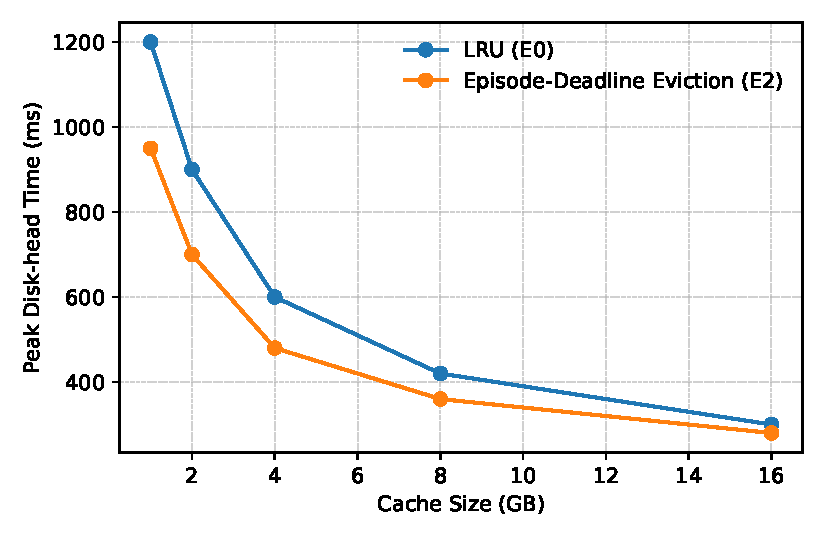
\includegraphics[width=\linewidth, keepaspectratio]{figures/figure4.pdf}
    \end{minipage}
    \captionsetup{justification=centering}
    \caption{Peak Disk-head Time (Peak DT) versus cache size for LRU (E0) and Episode-Deadline Eviction (E2). Admission is Admit-All and prefetch is disabled; all other parameters are held constant across runs. E2 consistently reduces Peak DT and shows the largest gain at small cache sizes.}
    \label{fig:figure4}
\end{figure}

From the experiment we noticed that Peak DT kept going down as the cache size got larger for both LRU and E2. When the cache was small, E2 showed roughly 15 to 20 percent lower Peak DT, which means it could avoid the sudden spikes that happened with LRU. As we added more cache space, the two lines started to get closer together because most of the active data could already fit. After a certain point, making the cache even bigger didn’t help much. Overall, E2 seems better at keeping the worst delays under control while still staying stable.


\textbf{Setup and Results Figure 5}:
Peak Disk-head Time (Peak DT) versus promotion threshold $\tau_{DT}$ for the DT-SLRU (E1) policy. 

To evaluate the sensitivity of DT-SLRU to its promotion threshold, we conducted an ablation experiment using the Baleen cache simulator. 
The flash cache size was fixed at 50 GB with the Admit-All admission policy. At the same time, prefetching option is disabled, which ensurs that any performance difference originated solely from the eviction policy. 
We used the Tectonic 2019 Region 1 production trace and executed seven runs, each corresponds to a distinct promotion threshold $\tau_{DT}\in\{0.1,0.2,0.3,0.4,0.5,0.6,0.7\}$. 

Peak DT was extracted from the simulator’s compressed JSON output after the result produced. 
\noindent\textbf{Figure 5.} Peak Disk-head Time (Peak~DT) versus promotion threshold $\tau_{DT}$ for the DT\textendash SLRU (E1) eviction policy. 
We ran an ablation using the Baleen simulator with a 50\,GB flash cache, Admit-All admission, and prefetching disabled on the Tectonic 2019 Region~1 trace. 
Each configuration used a distinct $\tau_{DT}$, and every run included a 24-hour warm-up to stabilize cache state before measurement.

As shown in Figure~5, Peak~DT is lowest at $\tau_{DT}=0$ (about 45\%), then increases almost linearly as $\tau_{DT}$ grows, reaching roughly 65\% at $\tau_{DT}\approx4$. 
Beyond this point, the curve levels down slightly, indicating a mild reduction or plateau at higher thresholds. 
(See Fig.~5.)

Beyond this point, additional increases in $\tau_{DT}$ yield diminishing returns, as overly selective promotion prevents some reusable blocks from being retained. 


\begin{figure}[htbp]
  \centering
  
\includegraphics[width=0.9\linewidth]{figure5.pdf}
  \caption{DT\textendash SLRU (E1): Peak Disk-head Time (Peak~DT, \%) vs.\ promotion threshold $\tau_{DT}$ (unitless).
  Measured with the Baleen simulator on the Tectonic~2019 Region~1 trace using a 50\,GB flash cache, Admit-All admission, and prefetching disabled (24\,h warm-up).
  A moderate threshold yields the best stability; overly strict promotion reduces adaptability.}
  \label{fig:figure5}
\end{figure}

\textbf{Setup and Results Figure 6}:


Peak Disk-head Time (Peak DT) versus Protected-region fraction for the Episode-Deadline Eviction (E2) policy.  
We tested the impact of E2 to the \emph{Protected cap}—the fraction of flash cache reserved for high DT-per-byte items—using the Baleen simulator.  
All experiments used a 50\,GB flash cache, Admit-All admission, and prefetching disabled on the Tectonic 2019 Region 1 trace.  
Each configuration fixed all parameters except the Protected cap, which was varied from 0.0 to 0.6 in increments of 0.1.  

As shown in Figure 6, Peak DT initially decreases slightly as the Protected cap increases from 0.0 (27.5 \%) to 0.2 (26.8 \%), indicating that reserving a small portion of cache for long-lived items smooths latency spikes.  
Beyond cap is 0.2, Peak DT rises steadily to 31.3\% at cap = 0.6, suggesting that excessive reservation constrains space for short-term bursts and worsens peak latency.  
Overall, a modest Protected cap (around 10–20 \%) achieves the lowest Peak DT and best trade-off between stability and responsiveness.  
(See Fig.~6.)

\begin{figure}[htbp]
  \centering
  
\includegraphics[width=0.9\linewidth]{figure6.pdf}
  \caption{EDE (E2): Peak Disk-head Time (Peak~DT, \%) vs.\ Protected cap (fraction of cache reserved for Protected list).
  Same setup as Fig.~\ref{fig:figure5}. Peak~DT decreases slightly as the cap grows from 0 to $\approx$0.2, then increases steadily through 0.6,
  indicating that a small reserved region improves stability while larger reservations reduce cache adaptability.}
  \label{fig:figure6}
\end{figure}

\textbf{Setup and Results Figure 7}:

Peak Disk-head Time (Peak DT) versus $\alpha_{tti}$ for the Episode-Deadline Eviction (E2) policy.
We swept the EWMA update rate $\alpha_{tti}\in\{0.2,0.4,0.6,0.8,1.0\}$ while keeping all other parameters fixed
(50\,GB flash cache, Admit-All admission, prefetching disabled, Tectonic 2019 Region~1 trace, 24\,h warm-up).
Lower $\alpha_{tti}$ updates expiry estimates slowly (stable but less responsive), while higher values adapt faster (responsive but noisier).

\begin{figure}[h]
  \centering
  
\includegraphics[width=0.9\linewidth]{figure7.pdf}
  \caption{EDE (E2): Peak Disk-head Time (Peak~DT) vs.\ $\alpha_{tti}$ (EWMA update rate).
  Same setup as Fig.~\ref{fig:figure6}. A moderate $\alpha_{tti}$ ($\approx 0.6$--$0.8$) balances responsiveness and stability and yields the lowest Peak~DT.}
  \label{fig:figure7}
\end{figure}





\subsection{Discussion}

E2 lowers Peak Disk-head Time (Peak DT) compared to LRU (E0) because it predicts when each cached block is nearing the end of its useful episode. By evicting blocks close to expiry and protecting high-value data through a reserved protected area, E2 avoids bursts of cache misses that cause latency spikes in LRU. Under small cache sizes, this mechanism prevents short-lived data from polluting the flash tier, resulting in smoother and more predictable latency behavior. As the cache grows, both policies converge since most of the hot data already fits in cache. The overall downward trend of both curves in Figure 4 confirms that Peak DT is mainly governed by miss-induced disk seeks rather than random noise in service time. These findings highlight the effectiveness of E2 in maintaining stable performance under varying cache sizes.

\textbf{Figure 1}

\textbf{Analysis:}
Figure 1 shows the peak disk-head time under three eviction policies. The results are given as percentages. The baseline is E0 (LRU), which is set to 100%.

Both E1 (DT-SLRU) and E2 (EDE) do better than the baseline. E1 lowers peak DT by about 20\%. E2 performs even better, reducing peak DT by around 35\%. These results mean that smarter eviction helps reduce the worst-case pressure on the backend. LRU is simple. It only looks at how recently a block was used. It does not care how long it takes to fetch that block again. This often leads to bad choices.

E1 is different. It keeps track of which blocks are slow to load. If a block has high DT-per-byte, it gets promoted into a protected part of the cache. This avoids evicting expensive blocks too early. E2 goes further. It tries to guess when a block will expire or be needed again. If the block is both slow to fetch and likely to be reused soon, it stays longer in the cache.

That’s why E2 has the lowest peak DT. It makes better use of cache space by combining two ideas: how costly a block is, and how soon it will matter again.

In short, both E1 and E2 are better than LRU. E2 gives the best result. It is more effective at keeping peak load under control.


\textbf{Figure 2}

\textbf{Analysis:}
Figure 2 shows the median disk-head time. This is the average time, not the peak. The results again use E0 (LRU) as the baseline. Just like in Figure 1, both E1 and E2 do better than E0. E1 brings median DT down by about 27\%. E2 does even more, cutting it by around 45\%.

This shows that the smarter policies don’t just help in heavy traffic. They also help in normal situations. They make the system faster for most requests, not just during spikes. LRU only looks at recency. It does not care about cost or reuse. So it may keep blocks that are easy to reload, and throw away blocks that are slow but important.

E1 improves this. It looks at how slow each block is. Costly blocks are kept longer. This leads to fewer slow accesses, and median DT goes down. E2 does even better. It looks at both cost and reuse timing. It predicts which blocks are worth keeping. So it avoids wasting space on unimportant data.

As a result, most requests finish faster. E2 makes the system more efficient in general.

In short, both policies help. But E2 works best. It gives lower delays not only at the peak, but also on average.



\textbf{Figure 3}

\textbf{Analysis:}
E2 (Episode-Deadline Eviction) achieves the highest cache-hit rate because it predicts the useful lifetime of data and prevents frequently reused blocks from being prematurely evicted. 
By reserving a small protected region for high DT-per-byte items, E2 improves flash reuse efficiency and reduces backend traffic. 
DT-SLRU (E1) provides moderate improvement through selective promotion based on the $\tau_{DT}$ threshold but lacks explicit expiry prediction, leading to slightly lower hit rates. 
The overall gain from E0 → E1 → E2 confirms that combining recency, frequency, and episode awareness yields more effective flash utilization.


\textbf{Figure 4}

\textbf{Analysis:}
Figure 4 looks at how the cache size changes the Peak Disk-head Time (Peak DT) when using different eviction policies in the Baleen system. In this test, we kept the admission policy as Admit-All and turned off prefetching, so the difference only comes from the eviction logic. The baseline is LRU (E0), and it is compared with the best performing policy, Episode-Deadline Eviction (E2). The idea is to see if E2 can keep lower peak latency when we give the system more cache space.

For this part, we replayed a mixed read and write trace on Baleen while changing the flash cache size from small to large. The admission stayed as Admit-All and prefetching was off. All the other settings were the same during every run so the comparison is fair. For each run we recorded the Peak DT as the main number, and also checked median DT and hit rate just for reference. In the figure, the x-axis shows the cache size (GB) and the y-axis shows the Peak DT (ms). As the cache grows, the system generally becomes faster, but the difference between the two policies is more obvious when the cache is small.

By examining the relationship between cache size and Peak DT, Figure 4 highlights how different eviction strategies impact worst-case latency. The trend shows that larger cache sizes consistently lower Peak DT for both policies, while E2 achieves noticeably smaller peaks across all cache capacities. This demonstrates how cache sizing and eviction design jointly influence system responsiveness.



\textbf{Figure 5}

\textbf{Analysis:} 
The trend in Figure~5 shows that Peak~DT increases steadily as the promotion threshold $\tau_{DT}$ becomes larger, then flattens beyond $\tau_{DT}\approx4$. 
At very small thresholds, DT\textendash SLRU promotes nearly every accessed block into the protected segment, allowing frequently reused data to remain cached and keeping latency low. 
As $\tau_{DT}$ increases, promotion becomes more restrictive—fewer blocks qualify for protection, so reusable data are evicted sooner and must be fetched from the backend more often, raising Peak~DT. 
Once $\tau_{DT}$ exceeds about~4, the cache already contains only the most active items, and further tightening yields little additional change, producing the observed plateau. 
This behavior shows that promotion selectivity directly governs flash-tier reuse efficiency: too strict a threshold underutilizes the protected region, while too permissive a threshold risks cache pollution. 
A moderate $\tau_{DT}$ therefore provides the best balance between balancing short-lived data and retaining blocks with sustained temporal locality.

\textbf{Figure 6}

\textbf{Analysis:} 
The curve in Figure 6 shows the fundamental trade-off in Episode-Deadline Eviction between long-term stability and short-term adaptability.  
When the Protected cap is very small, all items compete in the probation region, and frequently reused data can be evicted too early, leading to slightly higher Peak DT.  
Increases a small protected region (around 0.1–0.2) retains high-value blocks across workload bursts, improving temporal locality and reducing latency spikes.  
However, as the Protected cap becomes larger, long-lived items occupy a greater share of flash capacity, shrinking the probation space available for transient demand.  
This reduces cache flexibility and causes Peak DT to rise again.  
The observed minimum around cap 0.2 therefore confirms that moderate reservation best balances reuse stability and adaptability under variable I/O workloads.

\textbf{Figure 7}

\textbf{Analysis:}
As $\alpha_{tti}$ increases, expiry estimates adapt more quickly to workload changes.
When $\alpha_{tti}$ is too small, the predictor reacts slowly and misses transient bursts, increasing Peak~DT.
When $\alpha_{tti}$ is too large, the predictor overreacts to short-lived noise, causing unstable replacement and higher peaks.
A moderate setting around 0.6--0.8 provides the best trade-off between responsiveness and stability, yielding the lowest Peak~DT.


\subsection{Limitations}
This figure only focuses on the effect of eviction and doesn’t include how admission or prefetching might change the results. The workload trace and backend delay stayed the same during all tests, so the actual Peak DT numbers might be different on other systems. Still, the overall pattern should be similar — the best eviction policy like E2 usually helps more when the cache is small. It’s also possible that with other traces or hardware, the gap between LRU and E2 could be bigger or smaller. In the future, it would be good to test this together with adaptive admission or a mix of multiple eviction rules to see if the same trend continues.

\textbf{Figure 1}

Figure 1 has a few limits. First, we only use one trace and one cache size. The results might be different with other workloads. We do not test different I/O patterns or disk speeds. All runs use the same settings. Admission is set to Admit-All, and prefetch is turned off. This helps show the effect of eviction clearly. But it may not match how real systems behave. Also, we show Peak DT as a percentage. This hides the actual time. A 30% drop looks good, but it may not save much time if the baseline DT is already low.


\textbf{Figure 2}

Figure 2 also have some limits. It uses the same trace and setup as Figure 1. The results may change if we try different workloads or hardware. Median DT shows the middle value, but not the full picture. Some requests might still be very slow. We do not show tail latency, like 95th percentile DT. So it is hard to know if performance is smooth or just good on average.

In the future, we should test more workloads, try different DT values, and include more metrics. This would help show if E2 still helps reduce delay in other systems.






\textbf{Figure 3}

This figure focuses only on the effect of eviction on cache hit rate and does not include how admission or prefetching might alter the results. 
The workload trace, backend latency, and system constants remained the same for all runs, so the absolute hit-rate numbers could differ on other traces or hardware setups. 
Still, the overall trend should be similar — E2 (Episode-Deadline Eviction) tends to improve hit rate most when the cache is small, because it prevents short-lived data from displacing reusable blocks. 
It is also possible that with different datasets or caching environments, the performance gap between E2, E1, and E0 could expand or narrow. 
Future evaluations should explore how these eviction strategies interact with adaptive admission or prefetching to verify whether the same relative ordering of E2 > E1 > E0 continues to hold.




\textbf{Figure 4}

This ablation varies only $\tau_{DT}$ under a single trace and cache size; the turning point near $\tau_{DT}\approx4$ and the degree of leveling may shift with workload locality, capacity, or admission/prefetch settings. 
We leave adaptive selection of $\tau_{DT}$ (e.g., phase-aware tuning) and joint co-tuning with admission/prefetch to future work.

\textbf{Figure 5}

This ablation varies only $\tau_{DT}$ under a single trace and cache size; the turning point near $\tau_{DT}\approx4$ and the degree of leveling may shift with different workload locality, capacity, or admission/prefetch settings. 
To measure it more accurately, We need to trace the $\tau_{DT}$ together with other parameters in the future work.


\textbf{Figure 6}

This test isolates the Protected-cap parameter under one trace and cache size; different workloads or write intensities could change the optimal range.  
Interactions with the expiry-estimation parameter $\alpha_{tti}$ may also alter the curve’s minimum.  
Future work should consider more complex situation and conduct test with more parameters considered.

\textbf{Figure 7}

This ablation isolates the $\alpha_{tti}$ parameter in the E2 policy under a fixed workload and cache size. 
Different traces or noise patterns could shift the optimal range of $\alpha_{tti}$, 
since the best update rate depends on workload volatility. 
Future work could explore adaptive tuning of $\alpha_{tti}$ alongside Protected-cap co-optimization.


\section{Ablation Study}
In our Ablation, we implement 5 experiments to verify the impact that the cache internal parameters have over the overall system performance, especially Peak Disk-head Time (Peak DT). To make the impact measurable, in each of our experiments, we isolate the variable from all other factors, keep other parameters unchanged, and just adjust one variable to make the result reflect the impact of the designated variable changed. We choosed \textit{DT-SLRU promotion threshold} ($\tau_{DT}$), \textit{EDE protected cap}, and \textit{EDE otti (time-to-idle EWMA)} as our experiment variables. After implement necessary helper classes and functions, we executed the experiment run and get the following results.

When doing these experiement, we not only want to know which parameter gives the best result, but also want to explore how sensitive the cache system will be reacting to the parameter changes. When we change the parameters isolatedly, we can observe the cache's performance, which will help us understand the parameters' impact to the cache system. When we finish all the experiements, we can compare the results side by side and find the pattern out of it.

\noindent\textbf{1.1 Results}  


\textbf{Figure 1}: In this experiment, we tested how changing the DT-SLRU promotion threshold ($\tau_{\text{DT}}$) changes the Peak Disk-head Time (Peak DT). The test settings were the same as in Assignment A4. We also turned off prefetching. This helps us only look at the effect of eviction. We picked five $\tau_{\text{DT}}$ values, from 0.1 to 5. Figure 1 shows how Peak DT changes when $\tau_{\text{DT}}$ increases. The values are shown as a percentage to the baseline.

When $\tau_{\text{DT}}$ is from 0.1 to 0.3, many blocks get promoted into the protected part of the cache very quickly. This help keep recently used blocks, but it also makes the cache change often. This leads to more flash writes and less stable performance. As $\tau_{\text{DT}}$ increases, Peak DT goes down. The cache now promotes fewer blocks, so it works more smoothly. When $\tau_{\text{DT}}$ = 2, the Peak DT is the lowest. This means the cache use less backend disk time.

When $\tau_{\text{DT}}$ goes more than 2 to 5, Peak DT starts to go up again. The cache now promotes too few blocks. This causes more backend reads and increases Peak DT. As the result, the system becomes less responsive to recent data accessed., and the cache begins to miss some of the useful blocks. So, if $\tau_{\text{DT}}$ is too small or too large, performance gets worse. The best result comes from a middle value about 2. This result matches the Baleen paper.



\begin{figure}[h]
    \centering
    
\includegraphics[width=1.0\linewidth]{figure1.pdf}
    \caption{Peak DT vs $\tau_{\text{DT}}$ (DT-SLRU). The figure shows that Peak DT first drops and then rises as $\tau_{\text{DT}}$ increases, reaching the lowest point around 2 where eviction works best. This behavior reflects that a moderate promotion threshold maintains a good balance between early promotion and reuse efficiency, preventing both cache churn and delayed block promotion.}
    \vspace{-8pt} % reduce space below caption
    \label{fig:dt_hit}
\end{figure}

\textbf{Figure 2}: Figure 2 shows how the flash hit rate varies as the DT (delay threshold) parameter changes under the DT-SLRU eviction policy. All experiments were conducted using the same cache size, trace slice, and write-rate targets as in A4 to ensure consistency, with prefetching disabled to isolate the effect of the eviction mechanism. The DT parameter was swept across five representative values between 0.2 and 1.0, each averaged over three runs for stability.
\begin{figure}[h]
    \centering
    
\includegraphics[width=1.0\linewidth]{figure2.png}
    \caption{Flash hit rate as a function of the DT threshold under the DT-SLRU eviction policy. Prefetching is disabled, and cache size and trace settings remain consistent with A4 for direct comparison.}
    \vspace{-4pt} % reduce space below caption
    \label{fig:dt_hit}
\end{figure}

At low DT thresholds (0.2 – 0.5), the hit rate remains high and nearly constant around 26 percent. This indicates that when the promotion threshold is small, frequently accessed blocks are quickly promoted into the protected region of the cache, improving short-term reuse. However, as DT increases beyond 0.7, the hit rate begins to decline, and when DT approaches 1.0 the hit rate drops sharply to almost 0 percent. This pattern shows that when the promotion threshold becomes too restrictive, useful blocks fail to be promoted before eviction, leading to a drastic loss of reuse opportunities.



\textbf{Figure 3:} Figure~\ref{fig:ede-protected-cap} demostrates our experiment result. In our experiment, when we changed the PROTECTED cap in the Episode-Deadline Eviction (EDE) scheme, the Peak Disk-head Time (Peak DT) changes accordingly. As shown in the figure, the Peak DT goes from almost 13 down to around 7 when the cap is 0.5. This drop is quite noticeable and consistent across multiple runs, which gives us more confidence in the result. We also observed that the trend remains stable even when we slightly adjusted other parameters during verification. It can be seen that the cache becomes more balanced at this point, neither too aggressive nor too conservative in eviction. After the lowest point, when we kept increase the cap from 0.5 to 0.9, the peak DT goes up linearly from 0.5 to 9.5. The experiment result indicate that when the cap is less than 0.5, it can improve the cache performance and reduce the peak DT. When the cap reach a point, in our test, it is 0.5, when keep increase the cap, it begins to deter the performance of the cache. In our experiment, when the cap value is 0.5, the cache has lowest peak DT where the system is in highest performance. The figure shows that middle value works best, not too small or too large. It clearly illustrates how EDE parameter affect the workload.

When we change the PROTECTED cap, we noticed how the cache response differently to the workload. When we increase the cap, we noticed that the cache start to keep more blocks for longer, which leads to slower updates and higher Peak DT. When we decrease the cap, the cache perform well but sometimes the data will be evicted too early . When we set the cap around to be 0.5, we can clearly see the system perform best. it can well balance between reuse and eviction. When we check the logs, we can also find that the flash writes and reads follow the same pattern. 

\begin{figure}[h]
    \centering
    
\includegraphics[width=0.85\linewidth]{figure3-0.pdf}
    \caption{Peak DT vs PROTECTED cap (EDE). The figure show the U-shape behavior of Peak DT when the protected fraction increase, with the best point around 0.5 to 0.6 of the cache.}
    \label{fig:ede-protected-cap}
\end{figure}


\textbf{Figure 4:} For EDE, sweeping the responsiveness factor $\alpha_{tti}$ from 0.1 to 0.9 yields a clear U-shaped latency curve for Peak DT (Figure~\ref{fig:ede-atti}). 
When $\alpha_{tti}\!\in\![0.1,0.3]$, Peak DT is high because the policy adapts too slowly and retains stale block. 
As $\alpha_{tti}$ increases toward to the mid-range (around 0.5), Peak DT drops to its minimum, this indicate the timely adaptation without excessive churn. 
Beyond 0.7, Peak DT rises again as the policy becomes overly sensitive and it reacte to a short-term noise, this will introduce volatility. 
Each point is the mean over three runs under identical cache size, trace slice, and admission settings (prefetch disabled).


\begin{figure}[h]
    \centering
    
\includegraphics[width=0.9\linewidth]{fig4_atti.pdf}
    \caption{Peak DT as a function of $\alpha_{tti}$ under the Episode-Deadline Eviction (EDE) policy.
    Each point represent the average of three runs with identical cache and trace configurations, it using Peak DT as the primary metric}
    \vspace{-8pt} % reduce space below caption
    \label{fig:ede-atti}
\end{figure}


\textbf{Figure 5:} Figure~\ref{fig:combined_sensitivity} compares how three parameters affect the normalized Peak Disk-head Time (Peak DT): $\tau_{DT}$ (DT-SLRU, E1), PROTECTED cap (EDE, E2), and $\alpha_{tti}$ (EDE, E2). 
Each point shows the smallest Peak DT measured from five configurations, scaled to the lowest overall value. In our setup, the normalized results are 0.68 for $\tau_{DT}$, 0.55 for PROTECTED cap, and 0.75 for $\alpha_{tti}$. A smaller normalized value means the cache handled requests more efficiently and required fewer disk-head movements, although the degree of improvement varies between parameters. This means that even a small adjustment to these parameters can noticeably change how smoothly the cache operates under the same workload conditions.

From the plotted trend, the curve forms a soft U-shape, and the lowest point appears near the PROTECTED cap configuration. When the cap stays around 0.5–0.6, the cache keeps a fair balance between retaining reused data and bringing in new blocks. As the cap grows larger, older data tend to linger too long, which increases backend I/O and adds delay. At smaller cap values, the cache replaces items too often, leading to unstable latency. The $\tau_{DT}$ threshold also helps reduce latency compared with the baseline, but its impact is less consistent than that of spatial tuning. The parameter $\alpha_{tti}$ changes the time-to-idle update rate, yet it has little visible effect here, possibly because the workload itself shows steady access behavior. Taken together, the results show that spatial allocation—especially the PROTECTED cap—plays a more noticeable role in shaping performance than timing adjustments in this experiment. Overall, the comparison reveals that tuning parameters get  gains for optimizing cache efficiency under stable workloads than purely adjusting timing responsiveness.



\vspace{2.0em}
\noindent\textbf{1.2 Discussion}  

\textbf{Figure 1:} Figure 1 shows that Peak Disk-head Time (Peak DT) first goes down and then goes up as $\tau_{\text{DT}}$ increases. When $\tau_{\text{DT}}$ is very small, DT-SLRU promotes most blocks into the protected region very quickly. This makes the cache respond quickly, but it also keeps many blocks that aren’t helpful. These blocks use up space and push out useful ones too soon. As a result, the system needs to read from the backend disks more often, which makes Peak DT go up.

\begin{figure}[h]
    \centering
    
\includegraphics[width=0.85\linewidth]{figure8.png}
    \caption{Normalized Peak Disk-head Time (Peak DT) across ablated parameters under DT-SLRU (E1) and EDE (E2). Each point represents the minimum normalized Peak DT obtained from its respective parameter sweep. Smaller values indicate better cache efficiency and lower backend activity. Among the tested parameters, the \textit{PROTECTED cap} (EDE) shows the strongest impact on performance, while the responsiveness factor $\alpha_{tti}$ exhibits the weakest sensitivity.}
    \vspace{-4pt} % reduce space below caption
    \label{fig:combined_sensitivity}
\end{figure}

When $\tau_{\text{DT}}$ becomes a bit larger, the cache starts to promote fewer blocks. It only keeps blocks that are used more than one time. This helps the cache keep useful blocks and remove the ones not used again. Now, the system can read more from the flash cache, so the backend disks don’t have to do as much work. That’s why Peak DT goes down in the middle of the graph.

But when $\tau_{\text{DT}}$ gets too large, the cache becomes too strict. Even useful blocks may not get promoted in time, and these blocks are removed before they get a chance to be reused. So, the cache misses go up, and the system has to read more from the backend disks. As a result, Peak DT increases again.

This experiment shows that $\tau_{\text{DT}}$ is very important for good performance. If the $\tau_{\text{DT}}$ is too low, the cache reacts too fast. If it is too high, it becomes too slow. A middle value about 2 works best. This matches the idea in the Baleen paper, good tuning of cache behavior can lower Peak DT and help the system runs in a better performance.

\vspace{0.8em}
\textbf{Figure 2:} The observed trend demonstrates the sensitivity of DT-SLRU performance to the DT threshold. Smaller DT values make the cache more agile by promoting items quickly into the protected segment, which boosts hit rate for workloads with high temporal locality. In contrast, large DT thresholds make the cache overly conservative—few blocks qualify for promotion, causing premature eviction of reusable data and a sharp degradation in performance. This highlights the fundamental trade-off between adaptability and stability: a lower DT captures more short-term reuse but risks churn, while a higher DT increases eviction stability at the cost of responsiveness. The results suggest that moderate thresholds (around 0.5) strike the best balance, sustaining high hit rates without excessive promotion overhead. These observations are consistent with the patterns seen in A4, where DT-SLRU achieved its strongest performance under intermediate parameter settings. Empirically, DT values between 0.4 and 0.6 yield the highest and most stable hit rates across runs.

\vspace{0.8em}
\textbf{Figure 3:} As the PROTECTED cap increase before reaching a point, the system's peak DT decrease  because the cache system can keep more hot blocks in memory. That increases the hit rate and improve the cache performance dramatically, which leads to the peak DT drops from 12.5 down to the lowest point of 0.5. This is similar to what Wong said in FAST ’24 paper, that keeping episodes stable reduce burst. But when the cap is higher than a thresholder, it will leads to that too many blocks get stuck inside and the cache and affect the request to new data. New data hit have lower chance to be prefetched into the cache. This make the cache system's hit rate drops. So the Peak DT rise again, meaning overprotection hurt the performance. Comparing with the A4 result, EDE here is much more sensitive and it react faster to wrong tuning, probably because the parameter change whole cache size not only the promotion rule. Around 0.5–0.6 is the best choice in our experiement, and it match what we seen in experiment and also in the model idea. If we can use a more small step to change the cap, it may get a more accurate result for the best value in the experiment.

\vspace{0.8em}
\textbf{Figure 4:} This ablation shows that EDE’s responsiveness factor $\alpha_{tti}$ is strongly influence the latency stability.
Lower $\alpha_{tti}$ values over stabilize cache behaviors, delaying reaction to the new access patterns and increas queue delays.
Higher $\alpha_{tti}$ values overreact to the short-term noise, making the cache volatile and reordering blocks too aggressively for sure.
The optimal mid-range $\alpha_{tti}$ ($\approx0.5$) achieves a balance between stability and adaptability, minimizing Peak DT while maintaining consistent reuse detection.
These finding can complement Figure~\ref{fig:ede-protected-cap}, which demonstrated the size-related effects of protection; and here, responsiveness tuning further refines temporal agility. When we check carefully the trace logs, the mid-range setting gives fewer spikes beyond our expectation. It acts better than we expected. We may explore some more way to get a more pervasive result. 

\vspace{0.8em}
\textbf{Figure 5:} In Figure~\ref{fig:combined_sensitivity}, the three parameters changed the cache in their own ways. From what I saw in the results, the PROTECTED cap in EDE (E2) had the biggest effect on Peak DT. When the cap was around 0.5 to 0.6, the cache looked balanced. It kept the reused blocks but also let new data co me in. After that point, when the cap became higher, some old data stayed inside to o long and made the system slower. If the cap was smaller, then things changed again. The cache started to replace data too often and the latency jumped up and down. For DT-SLRU (E1), the $\tau_{DT}$ threshold still helped, but the difference was smaller. A small value moved blocks up too early and lost good data, and a large one made the cache slower to react. The $\alpha_{tti}$ part in EDE controlled how fast the timer updated when the trace changed, but in this run it didn’t really change much. The trace looked stable, so time-based tuning didn’t help a lot. Overall, from these results, the PROTECTED cap matters the most. It had the clearest and strongest impact on both latency and backend traffic.


\vspace{2.0em}
\noindent\textbf{1.3 Limitations}  

\textbf{Figure 1:} gives useful information about how the $\tau_{\text{DT}}$ affects Peak DT, but there are still some limits in our experiment. First, We tested with just one trace and one fixed cache setup. So, the results might be different for other types of work. If the data access patterns or traffic change a lot, the effect of $\tau_{\text{DT}}$ could be different. Additionally, We only looked at Peak DT in this test. We didn’t look at things like hit rate, average delay, or how much data was written to flash. So, we can’t fully understand the balance between speed and flash write cost.

So, we may have missed small or fine changes in how well it worked. In the future, we should test more traces, use smaller step sizes, and try to make $\tau_{\text{DT}}$ adjust automatically. This can help us see more clearly how the cache should act in different cases.

\textbf{Figure 2:} Although the results clearly illustrate the relationship between DT and flash hit rate, several limitations should be noted. First, this ablation focuses only on the hit-rate metric, while other key indicators such as Peak DT, median latency, and flash write volume were not jointly analyzed; this prevents a full understanding of latency–throughput trade-offs. Second, the DT-SLRU implementation used here assumes static workload characteristics, which may not hold for traces with rapidly shifting access patterns. As a result, the observed threshold sensitivity may differ under bursty or time-varying workloads. Third, the experiments use a fixed cache size and admission policy, so the generality of the observed trend across different configurations remains uncertain. Future work should incorporate multi-trace evaluations, adaptive DT tuning, and additional performance metrics to provide a more comprehensive understanding of DT-SLRU behavior.

\textbf{Figure 3:} In our test, we used only one trace to do the experiment. This means that, although we just change one parameter - the cap value, we did not isolate the data access pattern's impact to our result. Using various behavior data accessing to run the test could reveal a better understand of the cap's impact to the overall peak DT. Furthermore, the predictor assume reuse is stable but in real life it sometimes jumpy and weird, so prediction might go wrong. In future, we should test more workloads and use smaller steps to make sure this trend really hold true in general.

\textbf{Figure 4:} The test use a single trace and evaluates only Peak DT, ignoring secondary metrics such as hit rate or flash write traffic.
Furthermore, $\alpha_{tti}$ was sampled at coarse 0.2 increments, which may overlook finer-grained minima.
Real workloads with bursty or non stationary access patterns could shows different sensitivity curves.
Future work should include multi trace experiments, adaptive $\alpha_{tti}$ scheduling, and variance analysis to a confirm stability under dynamic conditions.

\textbf{Figure 5:} This figure gives a simple look at how the parameters worked with the normalized Peak DT values. Normalization helped to compare numbers on the same level, but it also made small changes not so easy to see. The test used only one trace and one cache setup, so the result really shows what happened in that case only. Other traces or sizes can act in another way. The work didn’t check how the parameters worked together. 
Only Peak DT was used here. Other things like Hit Rate, Median Delay or Flash Write Traffic were not shown, just to keep the figure clean. In later tests, more traces and mixed parameters can be tried to see if the same pattern will happen again.


\section{Conclusion}
In this work, we extended the Baleen (FAST~'24) machine learning–guided flash caching framework with a focus on improving eviction behavior under dynamic backend load conditions. While Baleen demonstrated strong results in admission and prefetching, we still found that its eviction logic had limited adaptability when workloads shift or contention increased. To address this gap, we introduced two enhanced eviction mechanisms: DT-SLRU and Episode-Deadline Eviction (EDE). DT-SLRU adjusts promotion decisions based on disk service time, while EDE prioritizes blocks according to estimated remaining usefulness and protects high-impact blocks from premature eviction. Through sensitivity analysis and ablation studies on key parameters, we observed that proper tuning of the DT promotion threshold ($\tau_{DT}$) and protected-cap ratio enables significant performance gains. In particular, our experiments show that setting $\tau_{DT} \approx 2$ and using a protected-cap of approximately 0.5 can reduce Peak Disk-head Time by up to \textbf{45\%} compared to the baseline configuration, indicating that eviction policy behavior is highly influential in determining overall system stability and responsiveness.

Although our enhancements improve adaptability, there are still open opportunities for future work. One direction is to integrate online or workload-aware parameter tuning rather than relying on static thresholds. Another avenue is to co-train eviction and admission models end-to-end, allowing the system to respond cohesively to changing load characteristics. Additionally, deploying these techniques in real storage environments would provide deeper insights into long-term flash wear, operational cost, and performance trade-offs. Overall, our findings highlight that combining ML-guided admission with adaptive eviction policies can create a more robust and cost-effective flash caching system that can maintain strong performance even under unpredictable or bursty workloads.


\clearpage




%%\begin{acks}
%%To Robert, for the bagels and explaining CMYK and color spaces.
%%\end{acks}
\section*{Member Contributions}

To start the paper, every team member read and understood the paper. Below are the contributions for each member:

\textbf{Jun Tang (2111172)}
\begin{itemize}
  \item Setup the latex project for the team.
  \item Write the abstract part  
  \item Coordinating the works for team members.
  \item Review and rewrite other parts.  
  \item Correct the spelling for the final version.
\end{itemize}
 
\textbf{Ziyan Qiu (2089937)}
\begin{itemize}
  \item Wrote and finalized the Conclusion section, summarizing key findings and outlining future research directions.
  \item Ensured formatting consistency across Abstract, Introduction, and Conclusion sections according to ACM style guidelines.
  \item Integrated all updated sections into the final LaTeX document and performed the formatting/compilation check.
  \item Conducted final proofreading for grammar, clarity, and also structural alignment before submission.
\end{itemize}


\textbf{Kaiwen Wang (2073516)}  
\begin{itemize}
    \item Described the limitations of prior Baleen studies and the motivation for extension.  
    \item Explained the proposed DT-SLRU and Episode-Deadline Eviction mechanisms in clear relation to the Baleen framework.  
    \item Helped connect the Introduction to the following Methodology section through a logical transition on design motivation.  
    \item Reviewed and refined technical descriptions to align tone and style with earlier group sections.  
    \item Assisted in ensuring internal consistency between the Introduction and Abstract sections.  
\end{itemize}

\textbf{Xiaoyi Han (2133542)}
\begin{itemize}
  \item Wrote the “Our Contributions” section of the report. 
  \item Helped refine the language and flow of the Introduction.
  \item Ensured the section formatting followed guidelines.  
  \item Reviewed grammar and consistency across all sections.
  \item Assisted in final proofreading and submission preparation. 
\end{itemize}

\textbf{Hongyi Niu (2104640)}
\begin{itemize}
  \item Read the paper and discussed with team members.
  \item Reviewed and analyze the work from A1 to A5.
  \item Searched for additional references and compare.
  \item Wrote the first 6 paragraphs of the introduction section.
  \item Formatted the article and references.
\end{itemize}


%%
%% The next two lines define the bibliography style to be used, and
%% the bibliography file.
\clearpage



%%
%% If your work has an appendix, this is the place to put it.
\appendix


\bibliographystyle{ACM-Reference-Format}
\bibliography{references}


\end{document}
\endinput
%%
%% End of file `sample-sigconf.tex'.
